\documentclass[12pt]{article}
\setcounter{secnumdepth}{6}

\usepackage{minted}
\usepackage{xspace} 
\usepackage{longtable}
\usepackage{tcolorbox}

%% Software name
\newcommand{\softwareFullName}{MFR (Macro Finance Research) Suite\xspace}
\newcommand{\softwareShortName}{MFR Suite\xspace}
\newcommand{\softwareNameProg}{mfr.\xspace}
\newcommand{\modelSolnProg}{mfr.modelSoln\xspace}
\newcommand{\jupyterWidgetsProg}{mfr.jupyterWidgets\xspace}
\newcommand{\sdmProg}{mfr.sdm\xspace}
\newcommand{\semProg}{mfr.sem\xspace}

%% Commands for folder name and link to download
\newcommand{\folderName}{\texttt{mfrSuite}\xspace}
\newcommand{\copyrightHolder}{Macro Finance Research (MFR) Team\xspace}
\newcommand{\linkToDownload}{\texttt{larspeterhansen.org}\xspace}

%% Commands for symbols in the paper
\newcommand{\wealthSymbol}{$W$\xspace}
\newcommand{\stochasticVolSymbol}{$V$\xspace}
\newcommand{\growthSymbol}{$Z$\xspace}
\newcommand{\idioVolSymbol}{$\widetilde{V}$\xspace}
\newcommand{\newbornRateSymbol}{$\nu$\xspace}
\newcommand{\deathrateSymbol}{$\lambda_d$\xspace}
\newcommand{\persistGrowthSymbol}{$\lambda_Z$\xspace}
\newcommand{\persistStochasticVolSymbol}{$\lambda_V$\xspace}
\newcommand{\persistIdioVolSymbol}{$\lambda_{\widetilde{V}}$\xspace}
\newcommand{\meanIdioVolSymbol}{$\bar{\widetilde{V}}$\xspace}
\newcommand{\meanGrowthSymbol}{$\bar{Z}$\xspace}
\newcommand{\meanStochasticVolSymbol}{$\bar{V}$\xspace}
\newcommand{\discountRateESymbol}{$\delta_e$\xspace}
\newcommand{\discountRateHSymbol}{$\delta_h$\xspace}
\newcommand{\TFPeSymbol}{$a_e$\xspace}
\newcommand{\TFPhSymbol}{$a_h$\xspace}
\newcommand{\inverseEISeSymbol}{$\rho_e$\xspace}
\newcommand{\inverseEIShSymbol}{$\rho_h$\xspace}
\newcommand{\adjCostSymbol}{$\phi$\xspace}
\newcommand{\riskAverESymbol}{$\gamma_e$\xspace}
\newcommand{\riskAverHSymbol}{$\gamma_h$\xspace}
\newcommand{\meanTFPVolSymbol}{$||\sigma_K||$\xspace}
\newcommand{\growthVolSymbol}{$||\sigma_Z||$\xspace}
\newcommand{\stochasticVolVolSymbol}{$||\sigma_V||$\xspace}
\newcommand{\idioVolVolSymbol}{$||\sigma_{\widetilde{V}}||$\xspace}
\newcommand{\equityConstraintSymbol}{$\underline{\chi}$\xspace}
\newcommand{\depreSymbol}{$\alpha_K$\xspace}

%% Commands for program names in the code
\newcommand{\wealthProg}{W}
\newcommand{\stochasticVolProg}{V}
\newcommand{\growthProg}{Z}
\newcommand{\idioVolProg}{Vtilde}
\newcommand{\newbornRateProg}{nu\_newborn\xspace}
\newcommand{\deathrateProg}{lambda\_d\xspace}
\newcommand{\persistGrowthProg}{lambda\_Z\xspace}
\newcommand{\persistStochasticVolProg}{lambda\_V\xspace}
\newcommand{\persistIdioVolProg}{lambda\_Vtilde\xspace}
\newcommand{\meanIdioVolProg}{Vtilde\_bar\xspace}
\newcommand{\meanGrowthProg}{Z\_bar\xspace}
\newcommand{\meanStochasticVolProg}{V\_bar\xspace}
\newcommand{\discountRateEProg}{delta\_e\xspace}
\newcommand{\discountRateHProg}{delta\_h\xspace}
\newcommand{\TFPeProg}{a\_e\xspace}
\newcommand{\TFPhProg}{a\_h\xspace}
\newcommand{\inverseEISeProg}{rho\_e\xspace}
\newcommand{\inverseEIShProg}{rho\_h\xspace}
\newcommand{\adjCostProg}{phi}
\newcommand{\riskAverEProg}{gamma\_e\xspace}
\newcommand{\riskAverHProg}{gamma\_h\xspace}
\newcommand{\meanTFPVolProg}{sigma\_K\_norm\xspace}
\newcommand{\growthVolProg}{sigma\_Z\_norm\xspace}
\newcommand{\stochasticVolVolProg}{sigma\_V\_norm\xspace}
\newcommand{\idioVolVolProg}{sigma\_Vtilde\_norm\xspace}
\newcommand{\equityConstraintProg}{chiUnderline\xspace}
\newcommand{\depreProg}{alpha\_K\xspace}
\newcommand{\nWealthProg}{nWealth\xspace}
\newcommand{\nGrowthProg}{nZ\xspace}
\newcommand{\nStochasaticVolProg}{nV\xspace}
\newcommand{\nIdioVolProg}{nVtilde\xspace}
\newcommand{\wealthMinProg}{wMin\xspace}
\newcommand{\wealthMaxProg}{wMax\xspace}

                
%% Packages
\usepackage{hhline}
\usepackage{hyperref}
\usepackage{tablefootnote}
%\usepackage[flushleft]{threeparttable}
\usepackage{threeparttablex}
\usepackage{listings}
\usepackage{amsmath,amssymb}
\usepackage{natbib}
\usepackage{mdframed}
\usepackage{xcolor}
\usepackage{matlab-prettifier}
\usepackage{graphicx}
\usepackage{grffile}
\usepackage[margin=1.0in]{geometry}
\usepackage[percent]{overpic}
\usepackage{float}
\usepackage{subfig}
\usepackage{color,soul}
%\usepackage[hidelinks]{hyperref}

%%
\newcommand\numberthis{\addtocounter{equation}{1}\tag{\theequation}}

%% Self-defined colors
\definecolor{lightblue}{rgb}{.8,.95,1}
\definecolor{LightBlue}{rgb}{.8,.9,1}
\sethlcolor{lightblue} 
\definecolor{codegreen}{rgb}{0,0.6,0}
\definecolor{codegray}{rgb}{0.5,0.5,0.5}
\definecolor{codepurple}{rgb}{0.58,0,0.82}
\definecolor{backcolour}{rgb}{0.95,0.95,0.92}

\renewcommand*\descriptionlabel[1]{\hspace\labelsep
                                \normalfont\bfseries
                                \sethlcolor{LightBlue}\hl{#1}}
\DeclareRobustCommand{\hlCODE}[1]{{\sethlcolor{backcolour}\hl{#1}}}



\title{\softwareFullName}
\author{Lars Peter Hansen, Joseph Huang, Paymon Khorrami, Fabrice Tourre\footnote{We would like to gratefully acknowledge the Macro Financial Modeling project through the generous financial support from the Alfred P. Sloan Foundation and Fidelity Investments and to thank Amy Boonstra, former MFM Executive Director, for her unconditional support. For their feedback, we thank Yu-Ting Chiang (University of Chicago), Jian Li (University of Chicago), Simon Scheidegger (HEC Lausanne), Elisabeth Proehl (University of Amsterdam), and conference participants at the 2nd MMCN, PASC18, University of Zurich, Northwestern University, and participants at the Economic Dynamics Working Group at the University of Chicago. We also would like to thank the Research Computing Center at the University of Chicago for their guidance on high performance computing, in particular Peter Carbonetto and Hossein Pourreza.}}
\date{Version: 0.1.2\footnote{If you have any questions, please contact: jhuang12@uchicago.edu, fabrice@uchicago.edu, paymon@uchicago.edu, hanxuh@uchicago.edu}}

\begin{document}
\nocite{*}
\maketitle
\begin{center}

\includegraphics[width=0.5\textwidth]{mfrLogo}
\end{center}

\tableofcontents

\newpage
\section{Introduction}

The \softwareFullName is a set of four user-friendly Python packages:

\begin{enumerate}
\item \texttt{\modelSolnProg}: provides model solution to the generalized framework introduced in \citet{HKT} (more in section \ref{modelSolnIntro})
\item \texttt{\sdmProg}: provides tools to compute stationary density given stochastic processes (more in section \ref{statDentIntro})
\item \texttt{\semProg}: provides tools to compute shock elasticities (more in section \ref{shockElasIntro})
\item \texttt{\jupyterWidgetsProg}: an auxiliary module that provides a Jupyter-based graphical user interface (GUI) that allows the user to visualize model results (more in section \ref{jupyterInter})
\end{enumerate}

\texttt{\sdmProg} and \texttt{\semProg} are independent modules and can be used without the other two. 

\subsection{License}

The software is distributed under the MIT License (please refer to file \texttt{/license/LICENSE.txt}). We kindly suggest that you cite the  \copyrightHolder and paper \cite{HKT}.

\newpage

\section{Installation}

\subsection{Installing \softwareShortName }
\paragraph{Step 1:} The setup and use of the \softwareShortName requires a Python 3 distribution with the \texttt{pip}
package manager. We recommend the Anaconda distribution (\href{https://www.anaconda.com/}{www.anaconda.com}), since it includes
the most relevant packages for scientific computation (even if you don't want to use Anaconda, we recommend that you install \texttt{miniconda} to manage your Python environment\footnote{It can be downloaded from \href{https://conda.io/miniconda.html}{https://conda.io/miniconda.html}}). If you decide not to use Anaconda, please ensure that you have installed the \texttt{numpy}, \texttt{scipy}, \texttt{matplotlib}, and \texttt{cython} packages before running anything else. \\

If you have not downloaded the \softwareShortName from \linkToDownload already, please do so. Afterwards, please unzip the file and you will end up with folder \folderName. Enter \folderName and continue by following the instructions below based on your operating system.

\subsubsection{Windows}
\paragraph{Step 2:}  If you've never compiled C++ code on your computer before, you probably need to install a C++ compiler. To do so, we recommend that you install Microsoft Visual Studio 2017 (\href{https://visualstudio.microsoft.com/downloads}{https://visualstudio.microsoft.com/downloads}). After you download and open the installer, please select \textit{Visual Studio Community 2017} (figure \ref{fig:windowsVS}). When choosing which development package/environment/toolkit, select only \textit{Linux development with C++} (figure \ref{fig:windowsC}). Note: although the core code of the \softwareShortName is written in C++, you don't need any knowledge of C++ to use the software.

\begin{figure}[H]
\centering
\begin{minipage}{.5\textwidth}
  \centering

\includegraphics[scale=0.4]{windowsVSInstaller}
  \captionof{figure}{Choosing Visual Studio}
  \label{fig:windowsVS}
\end{minipage}%
\begin{minipage}{.5\textwidth}
  \centering

\includegraphics[scale=0.4]{windowsC}
  \captionof{figure}{Choosing Linux}
  \label{fig:windowsC}
\end{minipage}
\end{figure}

\paragraph{Step 3:} You may need to upgrade your \texttt{pip} to the newer version (such as 18.1). To do so, open up the Anaconda command prompt (not the command prompt that you get by typing in \texttt{cmd}) and run \texttt{pip install --upgrade pip}.

\paragraph{Step 4:} After upgrading pip, in the Anaconda command prompt, go into the folder of the \softwareShortName. Run the installation batch file by running \texttt{install.bat} in the Anaconda prompt. Depending on the Python version you're using, you might see an error. Please refer to section \ref{sec:potentialError} for a solution.

\paragraph{Step 5:} The installation process is now complete. If the installation was successful, you should see the following message:\\
 \begin{tcolorbox}[colback=green!5!white,colframe=green!75!black]
 mfr.sem was installed successfully.\\\
  mfr.sdm was installed successfully.\\\
  mfr-modelSoln was installed successfully.\\\
  mfr-jupyterWidgets was installed successfully.\\\
  modelSolnCore was installed successfully.
  \end{tcolorbox}

If not, you would see an error message suggesting which package was not installed successfully. For example, you could see:\\
\begin{tcolorbox}
========================================\\\
ERROR: mfr.sdm WAS NOT INSTALLED SUCCESSFULLY.\\\
Re-run `pip install ./src/sdm' in the command line and \\\
look for explanation in documentation on common errors.\\\
========================================
  \end{tcolorbox}
  
If you do see such an error message, run the command as suggested and see the related error. Afterwards, look for a solution in section \ref{sec:potentialError}. \\

If the installation was successful,  for a quick start guide, please refer to section \ref{quickStart}. If you wish to test models without doing any coding, please try out the graphical user interface in section \ref{jupyterInter}.

\subsubsection{macOS/Linux}

\paragraph{Step 2:} If you've never compiled C++ code on your computer before, you probably need to install a C++ compiler. To check, run \hlCODE{\texttt{g++}} in the Terminal. If you already have a C++ compiler set up, you would see a message similar to \texttt{clang: error: no input files}. If not, the Terminal should prompt you to install XCode command line tools (figure \ref{fig:xcodeCommand}). If the Terminal does not prompt you to install XCode command line tools, you can run \hlCODE{\texttt{xcode-select --install}} and you would see the same prompt as in figure \ref{fig:xcodeCommand}.

\begin{figure}[H]
\centering

\includegraphics[scale=0.4]{xcodeCommand}
\caption{Installing command line tools for macOS}\label{fig:xcodeCommand}
\end{figure}

If you use Linux, you can run \hlCODE{\texttt{sudo apt-get install build-essential}} in the terminal. If you have compiled C++ code before, you can skip this step. Note: although the core of the \softwareShortName is written in C++, you don't need any knowledge of C++ to use the software.

\paragraph{Step 3:} Open up Terminal and  \hlCODE{\texttt{cd}} into the software folder. Run the \texttt{install.sh} script to install the Suite (you can use  \hlCODE{\texttt{./install.sh}} in the Terminal). Depending on the Python version you're using, you might see an error. Please refer to section \ref{sec:potentialError} for a solution.

\paragraph{Step 4:} The installation process is now complete. If the installation was successful, you should see the following message:\\
 \begin{tcolorbox}[colback=green!5!white,colframe=green!75!black]
 mfr.sem was installed successfully.\\\
  mfr.sdm was installed successfully.\\\
  mfr-modelSoln was installed successfully.\\\
  mfr-jupyterWidgets was installed successfully.\\\
  modelSolnCore was installed successfully.
  \end{tcolorbox}

If not, you would see an error message suggesting which package was not installed successfully. For example, you could see:\\
\begin{tcolorbox}
========================================\\\
ERROR: mfr.sdm WAS NOT INSTALLED SUCCESSFULLY.\\\
Re-run `pip install ./src/sdm' in the command line and \\\
look for explanation in documentation on common errors.\\\
========================================
  \end{tcolorbox}
  
If you do see such an error message, run the command as suggested and see the related error. Afterwards, look for a solution in section \ref{sec:potentialError}. \\

If the installation was successful,  for a quick start guide, please refer to section \ref{quickStart}. If you wish to test models without doing any coding, please try out the graphical user interface in section \ref{jupyterInter}.

\subsubsection{Optional Step (for Exporting Plots as Files with \texttt{Plotly})}\label{sec:optionalPlotting}
The \texttt{\modelSolnProg} module uses either \texttt{matplotlib} or \texttt{plotly}, another plotting engine, to generate plots. By default (with the exception of the GUI discussed in section \ref{jupyterInter}), the module uses \texttt{matplotlib} to display plots or export plots into files. However, if you would like to export \texttt{Plotly}-generated plots into files (for example, if you would like to use \hlCODE{\texttt{.dumpPlots(fancy = True)}}, which exports plots into files, as described in section \ref{section:otherMethods}), you need to implement this section\footnote{This section is only necessary when you want to \textit{export} plots into files with \texttt{plotly}. If you want to display plots on the screen with \texttt{plotly}, this section is not needed. You only need to run the module in an interactive environment, such as Jupyter, if you want to display \texttt{plotly}-based plots on the screen.}. \\

This section contains the steps to install two packages, \texttt{plotly-orca} and \texttt{psutil}. If you use the Anaconda distribution (or miniconda), you can simply run the following command in the Terminal if you use macOS or Linux, or the Anaconda prompt if you use Windows:\\

\hlCODE{\texttt{conda install -c plotly plotly-orca psutil}}\\

If you don't use the Anaconda distribution, please refer to \href{https://plot.ly/python/static-image-export/}{this link} and follow the instructions in \textit{npm + pip} or \textit{Standalone Binaries + pip}.
\subsubsection{Potential Errors}\label{sec:potentialError}
We use \texttt{pip} to install packages but some existing packages might have been installed by \texttt{disutils} and could create confusion for \texttt{pip}. For example, you might see an error such as:\\

\begin{tcolorbox}Cannot uninstall `traitlets'. It is a distutils installed project and thus we cannot accurately determine which files belong to it which would lead to only a partial uninstall.
\end{tcolorbox}
\begin{tcolorbox}
Cannot uninstall `llvmlite'. It is a distutils installed project and thus we cannot accurately determine which files belong to it which would lead to only a partial uninstall.
\end{tcolorbox}

These two errors are essentially the same, except for the involved package.
If you see the same or similar error, you need to manually uninstall the package located in \texttt{site-packages} of Python's directory. To do so, follow the steps below (suppose the conflicted package is \texttt{llvmlite}):

\begin{itemize}
\item Find your Python's \texttt{site-packages} directory: in the Terminal, run \hlCODE{\texttt{python -c "import site; print(site.getsitepackages())"
}}. This command would give you the path of the \texttt{site-packages} directory (for example, the directory could be \\\ \texttt{/anaconda3/lib/python3.5/site-packages}). Enter the directory by doing, for example, \hlCODE{\texttt{cd /anaconda3/lib/python3.5/site-packages}}.
\item Delete folder \texttt{llvm-0.x.x} (the \texttt{x}s in \texttt{0.x.x} are variable, depending on the version number; for example, the folder could be called \texttt{llvmlite-0.26.0}) by doing, for example,  \hlCODE{\texttt{rm -r llvmlite-0.26.0}}.
\item Delete egg file \texttt{llvmlite-0.26.0-py3.5.egg-info} (note that the numbers in the file name could look different depending on your versions) by doing \hlCODE{\texttt{rm llvmlite-0.26.0-py3.5.egg-info}}.
\end{itemize}

You may then attempt to re-run the installation file (\texttt{install.sh} or \texttt{install.bat}).

\subsection{Quick Start Guide}\label{quickStart}

We've included a few examples for you to get started (you can find a more detailed explanation on the examples in section \ref{examplesSec}). To quickly solve a one-dimensional model, please go into the \texttt{examples} folder and run \texttt{test1DModel.py}. You can try \texttt{test2DModel.py} and \texttt{test3DModel.py} for two-dimensional and three-dimensional models respectively.\\

If you are interested in computing stationary density and shock elasticities, you can use \texttt{HeKrushnamurthy.py} and \texttt{BansalYaron.py}. These two scripts compute the stationary density and shock elasticities of two models.

\newpage
\section{Graphic User Interface}\label{jupyterInter}

\subsection{Start the Interface}
The Suite comes with a graphical user interface (GUI) that allows you to solve models by inputting your own parameters and compute the stationary density and shock elasticities of a solved model, \textit{without any coding at all}. The GUI is built on \textit{Jupyter}, a Python extension (no knowledge of \textit{Jupyter} is needed). If you used the Anaconda distribution as suggested, you already have Jupyter set up and are good to go. If not, you would need to follow the instructions \href{https://jupyter.org/install}{here}. \\

After getting Jupyter set up, open up Terminal (if you use macOS/Linux) or the Anaconda Prompt (if you use Windows), and \texttt{cd} into the \texttt{examples} folder. Run \texttt{jupyter-notebook}. This command will open up Jupyter in your browser. Click \texttt{Python Jupyter Interface.ipynb} as indicated in figure \ref{clickOpenJupyter}. (Note: you can copy \texttt{Python Jupyter Interface.ipynb} into a location that you prefer; the file can be stored and called anywhere).

\begin{figure}[H]
\centering
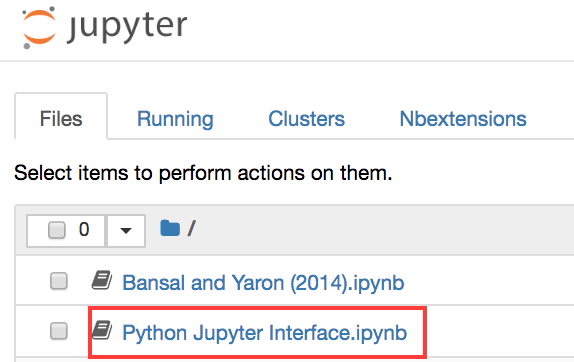
\includegraphics[scale=0.5]{jupyterScreenshot}
\caption{Start the GUI}\label{clickOpenJupyter}
\end{figure}

After opening the file, you will see an uninitialized interface (figure \ref{fig:uninit}). Click \textit{here} as shown in the red box. You then see the underlying code. Select the first cell with Python code (as boxed in red in figure \ref{fig:init}) by clicking the cell. After that, click button \textit{Run} (as boxed in blue in figure \ref{fig:init}). The notebook is then initialized and ready to use.

\begin{figure}[H]
\centering
\begin{minipage}{.5\textwidth}
  \centering
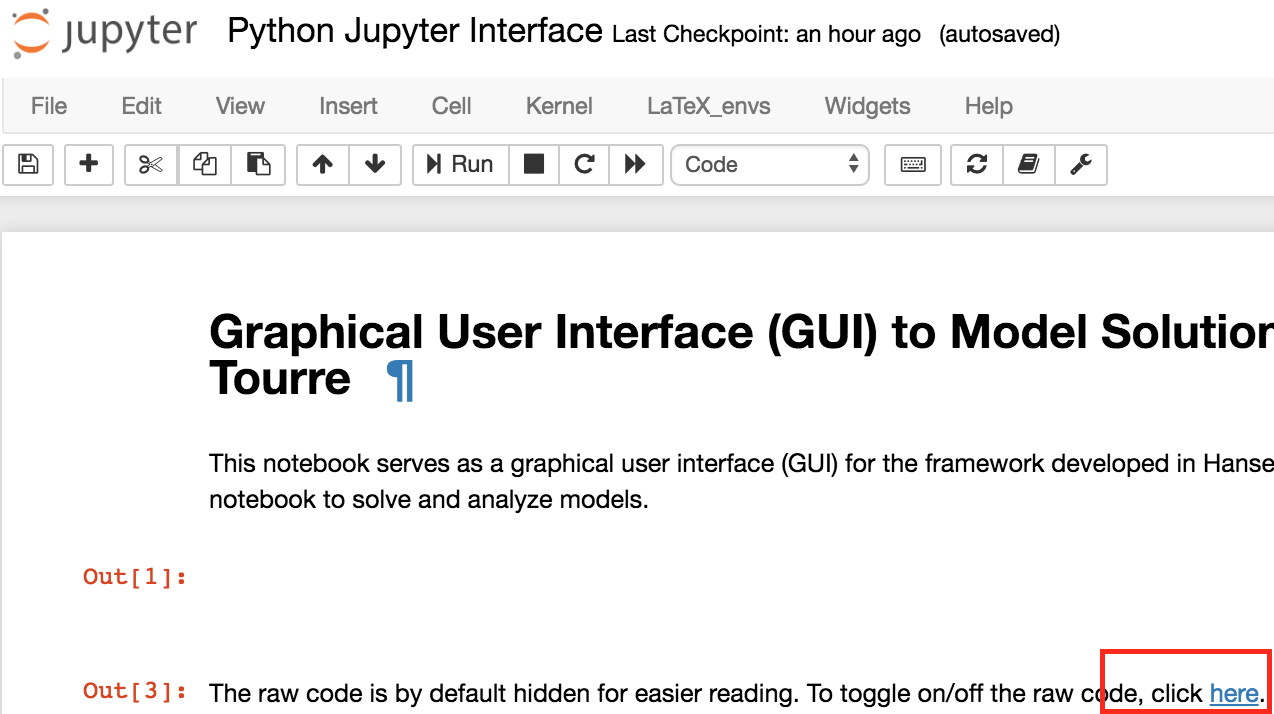
\includegraphics[scale=0.3]{jupyterNotebookBefore}
  \captionof{figure}{Uninitialized notebook}
  \label{fig:uninit}
\end{minipage}%
\begin{minipage}{.5\textwidth}
  \centering
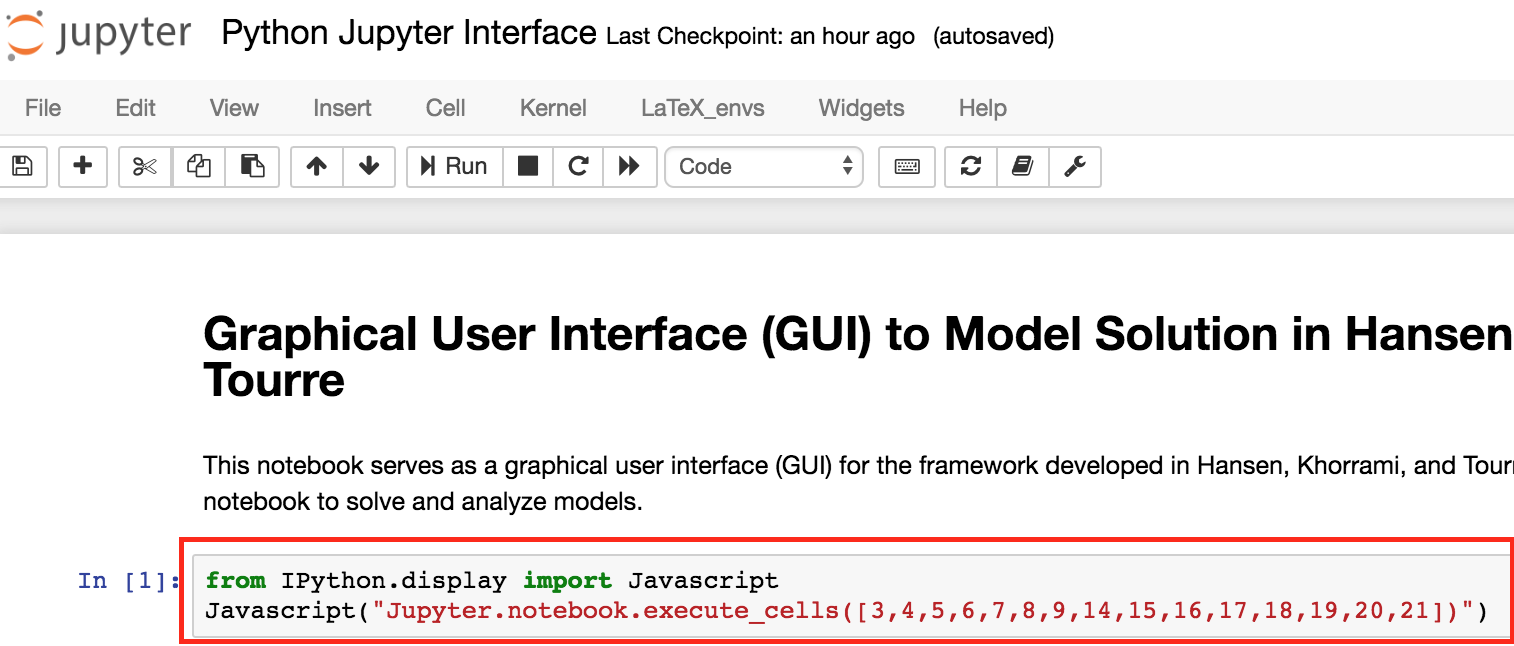
\includegraphics[scale=0.35]{jupyterDisplayed}
  \captionof{figure}{Initializing the notebook}
  \label{fig:init}
\end{minipage}
\end{figure}

\subsection{Solving a Model}

\paragraph{Solving a model} After initializing the notebook, you can start solving models by inputting your parameters (figure \ref{fig:setParams}). By default, the parameters will lead to a one-dimensional model with log-utility agents. A detailed explanation on the parameters can be found in section \ref{setParams}.

\begin{figure}[H]
\centering
\begin{minipage}{.5\textwidth}
  \centering
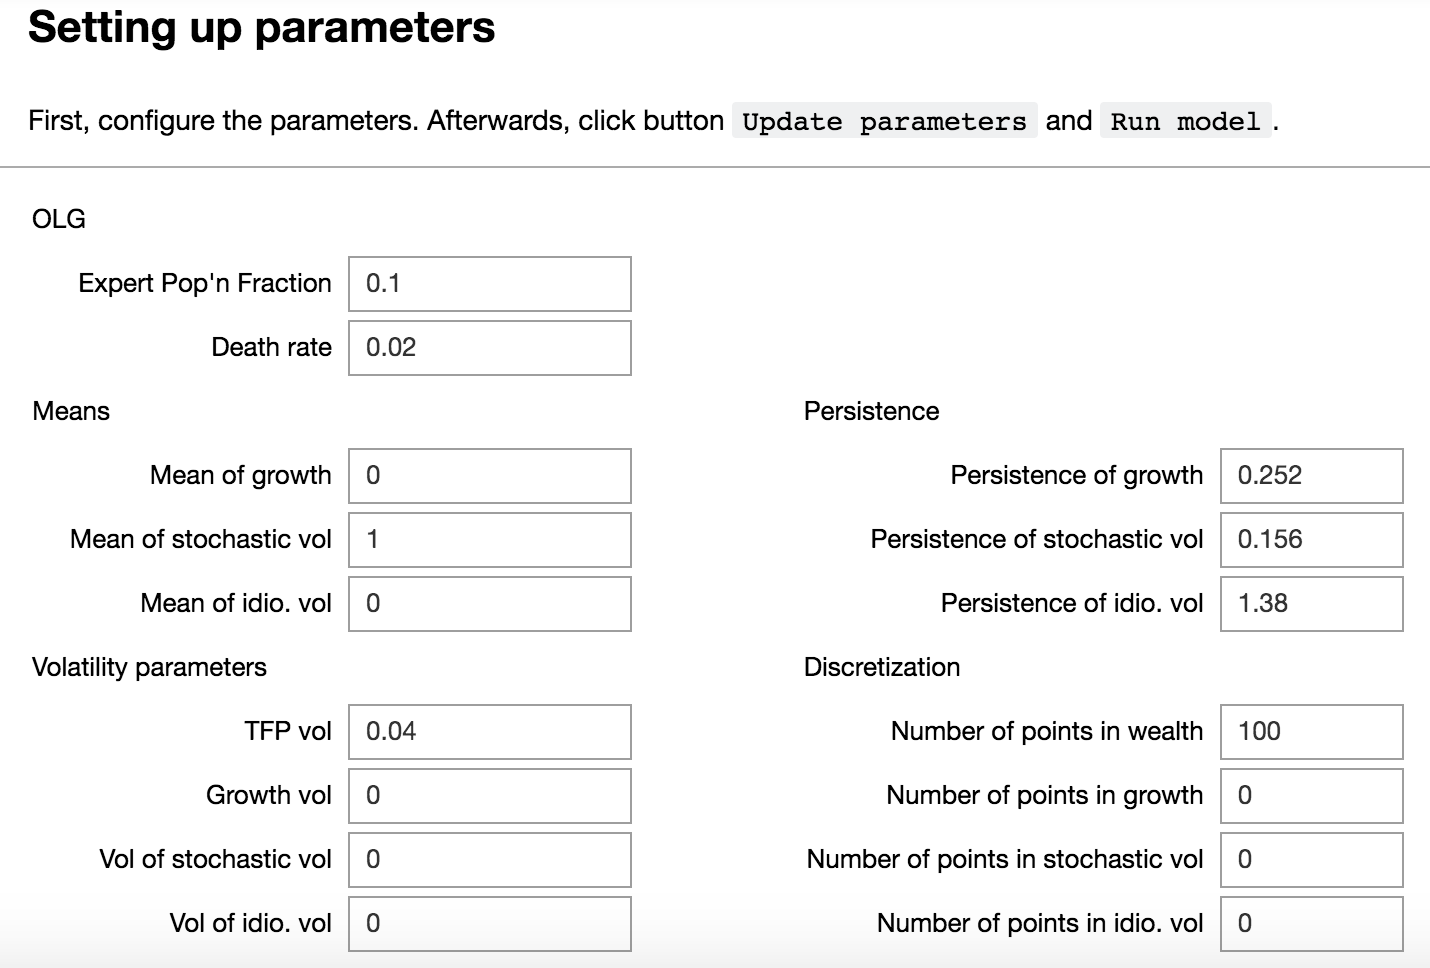
\includegraphics[scale=0.2]{settingParams}
  \captionof{figure}{Inputting parameters}
  \label{fig:setParams}
\end{minipage}%
\begin{minipage}{.5\textwidth}
  \centering
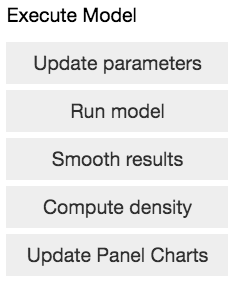
\includegraphics[scale=0.5]{jupyterButtons}
  \captionof{figure}{Buttons to solve models}
  \label{fig:buttons}
\end{minipage}
\end{figure}

When you finish inputting your parameters, you can solve and analyze the model by using these five buttons (figure \ref{fig:buttons}):
\begin{itemize}
\item \textit{Update parameters}: update the parameters of the model using your input. If you don't click this button after modify the parameters, the interface will not register your change.
\item \textit{Run model}: solve the model.
\item \textit{Smooth results}: after solving a model with capital misallocation, you may or may not need to smooth equilibrium quantities $\kappa$ and $q$.
\item \textit{Compute density}: compute stationary density of the model \textit{after} it is solved.
\item \textit{Display charts}: visualize the model results. Note that this button can be used without computing stationary density.
\end{itemize}

For example, after solving a 2D model, you can click \textit{Display charts} and one of the equilibrium quantities (functions of two state variables), \textit{Experts' Equity Retention}, would be visualized as in figure \ref{fig:viz2d}.

\paragraph{Stopping the solution program.} If you wish to terminate the model solution after clicking \textit{Run Model}, (for example, if it is taking too much time and you wish to adjust the parameters), you may click the stop button (on top of the GUI) as in figure \ref{fig:buttonStop}. Alternatively, you may click \textit{Kernel} and then \textit{Interrupt} as in figure \ref{fig:interruptKernel}. These two options are equivalent.\footnote{These options do not apply if you use Windows, as Jupyter does not throw the recognizable Windows signal, \texttt{CTRL\_C\_EVENT}. To terminate the program, you have to kill the kernel. However CTRL+C still works if you are using Python directly, regardless of the operating system.}

\begin{figure}[H]
\centering
\begin{minipage}{.5\textwidth}
  \centering

\includegraphics[scale=0.6]{buttonStop}
  \captionof{figure}{Clicking stop button}
  \label{fig:buttonStop}
\end{minipage}%
\begin{minipage}{.5\textwidth}
  \centering
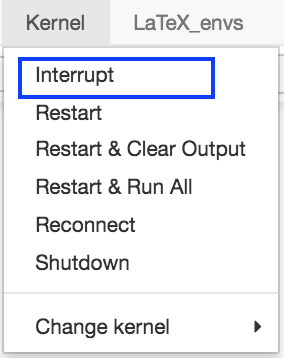
\includegraphics[scale=0.5]{menuInterrupt}
  \captionof{figure}{Interrupting the kernal}
  \label{fig:interruptKernel}
\end{minipage}
\end{figure}

After stopping the program, a message will show up and let you know the location of the \texttt{log.txt} file, which contains the history of the program (for a more detailed discussion of this file, please refer to section \ref{sec:logfile}).

\begin{figure}[H]
\centering
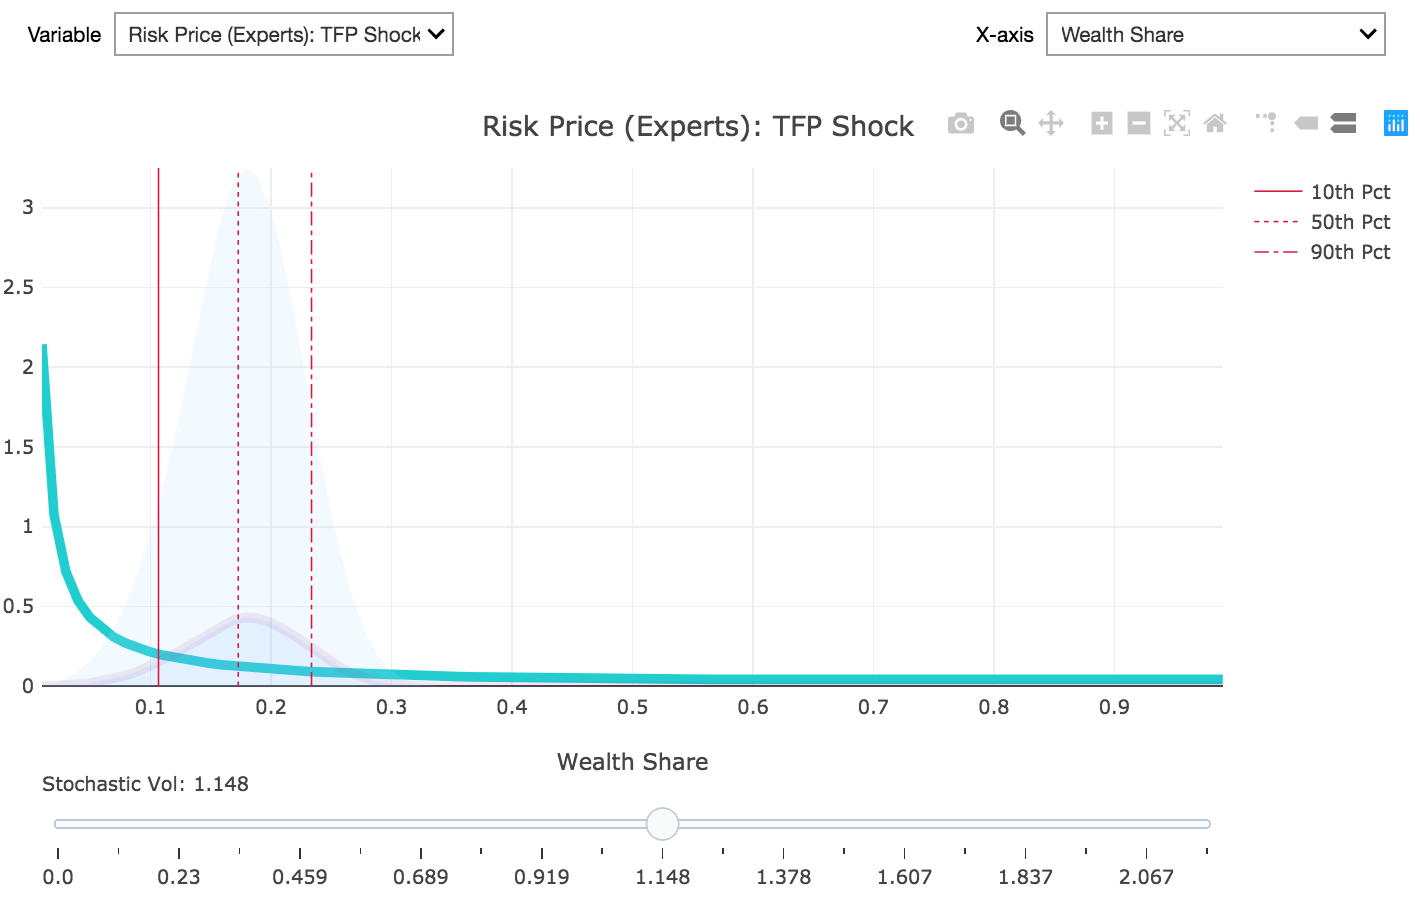
\includegraphics[scale=0.4]{sliderJupyter}
\caption{Visualizing an equilibrium quantity from a two-dimensional model. In this chart, the equilibrium quantity is a function of two state variables, one of which, wealth share, is on the x-axis, whereas the other, stochastic volatility, is on the adjustable slider. The 1D plot shows the equilibrium quantity as a function of wealth share, fixed at a specific point of stochastic volatility.}\label{fig:viz2d}
\end{figure}

\subsection{Analyzing a Model}
After solving a model, you may compute its stationary density by clicking button \textit{Compute density}. Afterwards, you may compute the ergodic mean, standard deviation, and correlations of the equilibrium quantities using the functionalities in section \textit{Diagnostics} (fig \ref{fig:compMoments}). Similarly, you may compute and visualize shock elasticities by perturbing a selected list of equilibrium quantities (figure \ref{fig:compElas})

\begin{figure}[H]
\centering
\begin{minipage}{.5\textwidth}
  \centering
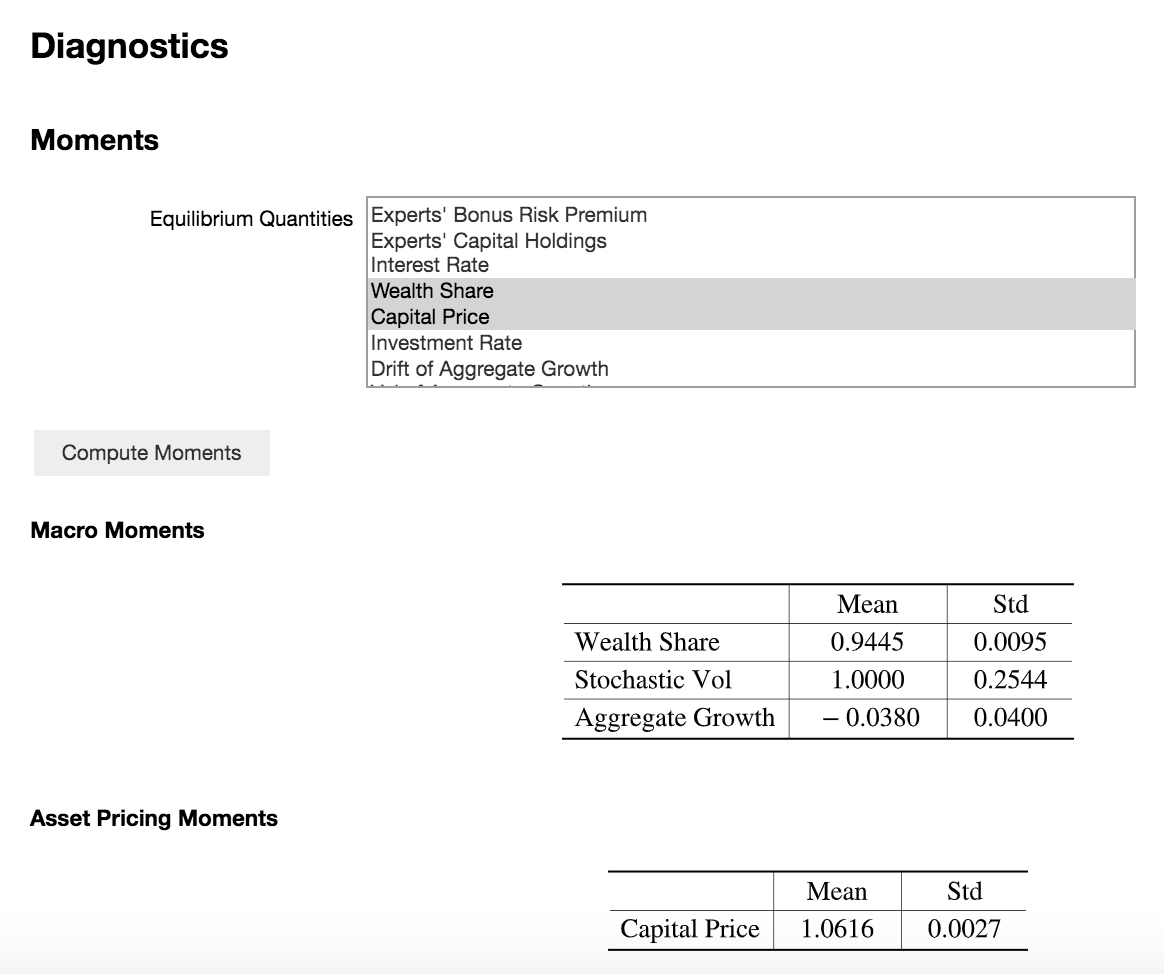
\includegraphics[scale=0.3]{moments}
  \captionof{figure}{Computing moments}
  \label{fig:compMoments}
\end{minipage}%
\begin{minipage}{.5\textwidth}
  \centering
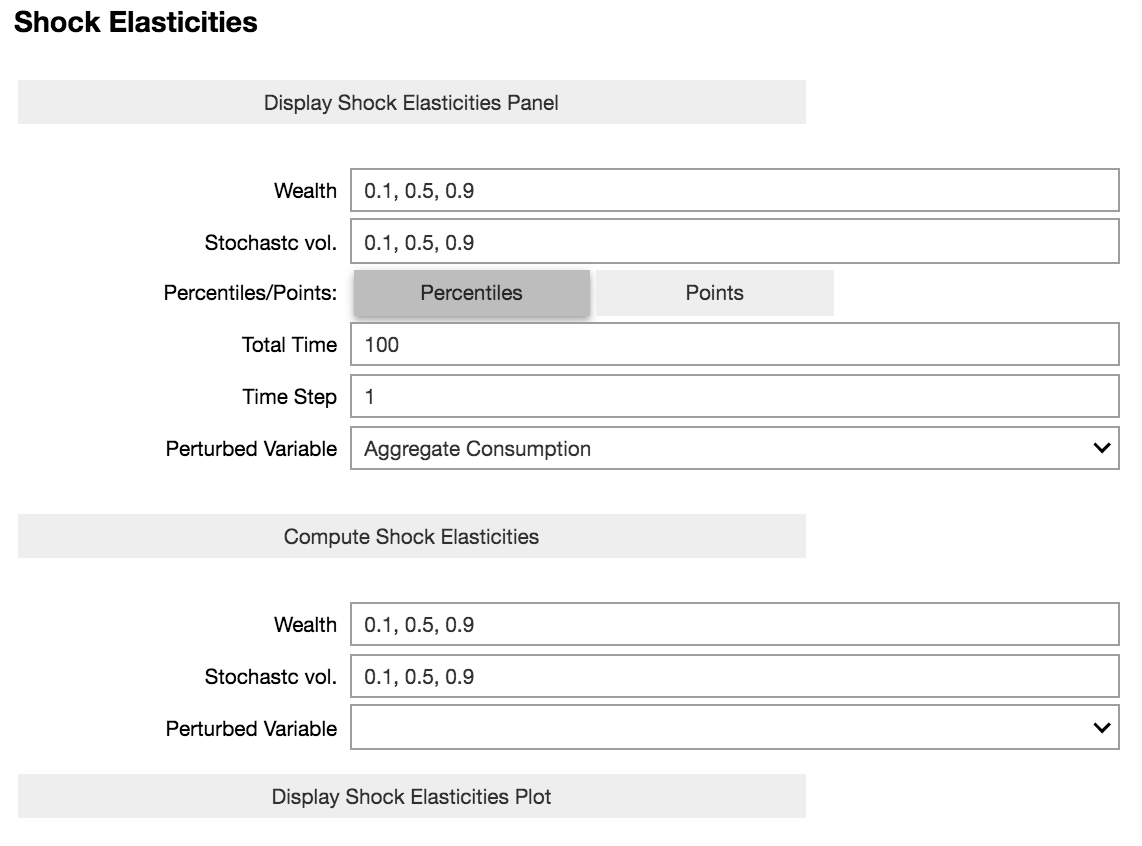
\includegraphics[scale=0.3]{shockelas}
  \captionof{figure}{Computing Shock Elasticities}
  \label{fig:compElas}
\end{minipage}
\end{figure}

\subsection{Comparing Models and Advanced Usage}
Note that the notebook \texttt{Python Jupyter Interface.ipynb} does not have any location dependence. That is, you can copy this file anywhere. To compare different models, you can simply duplicate this file and run two notebooks simultaneously. We advise against running the same notebook in two different browser windows, as it would create a conflict.\\

If you are familiar with Python and Jupyter and would like to modify a computed model, you can create a new cell below the notebook (or modify the notebook however you'd like). The underlying object behind the GUI is \texttt{defaultModel}. You can call the methods of this object as discussed in section \ref{HKTtools}. For example, you can use \texttt{defaultModel.plot(`q')} to plot the capital price.

\newpage

\section{Generalized Modeling Framework in Hansen, Khorrami, and Tourre} \label{modelSolnIntro}

\texttt{\modelSolnProg} solves the framework developed in \citet{HKT}: a dynamic stochastic general equilibrium model featuring two types of agents: experts, which we think of as financial intermediaries and households. We built from the original framework of \citet{BS2014}, to which we add a constellation of shocks and for which we use generalized recursive preferences. Note that while \texttt{\modelSolnProg} depends on the independent stationary density and shock elasticities toolboxes in section \ref{sec:otherTools}, you don't need to go through this section to use the stationary density and shock elasticities toolboxes in section \ref{sec:otherTools}.\\

\subsection{Model Overview}
Our agent types might differ in their productivities, their attitudes towards risk, their ability to smooth consumption inter-temporally, and their access to financial markets. Both agent types can hold physical capital to produce consumption goods according to a standard linear production technology. Capital holdings expose agents to a constellation of idiosyncratic and aggregate shocks, described in this model overview.

\subsubsection{Preferences}

\begin{itemize}
 \item Two types of agents in our economy: ``experts'' (subscript ``$e$'') and ``households" (subscript ``$h$'')
 \item Each group features a continuum of measure 1 of agents
 \item Consider a ``representative'' expert and a ``representative'' household
 \item Each agent type $j$ has recursive (``Kreps-Porteus'') preferences over consumption streams.  
 \item Overlapping generation structure: 
 \begin{itemize}
  \item Agents die and are borne at a constant Poisson rate \deathrateSymbol.
  \item Wealth of dying agents is distributed to new-born agents, a fraction \newbornRateSymbol being given to experts and a fraction $1-\nu$ being given to households. 
 \end{itemize}
  \item Consumption and continuation values of agent $j$ are denoted by $C_{j,t}$ and $U_{j,t}$, respectively, where the continuation value satisfies the continuous time counterpart to the following discrete time recursion:
\begin{align} \label{discrete_recursion}
U_t &= \left[ \left[ 1 - \exp( - \delta \epsilon ) \right]\left(C_t\right)^{1 - \rho} + \exp( - \delta \epsilon) {\mathbb R}(U_{t+\epsilon} \mid {\mathcal F}_t  )^{1 - \rho} \right]^{\frac 1 {1 - \rho}} \cr
 {\mathbb R}(U_{t+\epsilon} \mid {\mathcal F}_t ) & = \left(  \mathbb{E}  \left[ \left(U_{t+\epsilon} \right)^{1-\gamma} \mid {\mathcal F}_t \right]\right)^{\frac 1 {1-\gamma}}
\end{align}
 parameterized by: 
 \begin{itemize}
  \item A rate of time preference $\delta_j$
  \item A relative risk aversion coefficient $\gamma_j$
  \item An elasticity of inter-temporal substitution $1/\rho_j$
 \end{itemize}
\end{itemize}

\subsubsection{Technology}

\begin{itemize}
\item Capital $K_{j,t}$ of agent type $j$ evolves as:
\begin{align*}
 dK_{j, 
 t} &= K_{j,t} \left[ \left( Z_t + \Phi(I_{j,t}) - \alpha_K \right)dt + \sqrt{V_t} \sigma_K \cdot dW_t + \sqrt{\widetilde{V}_t} \cdot d\widetilde{W}_t \right]  
\end{align*}
where $I_{j,t}$ is the investment capital ratio.  
\item Exogenous state variables $\{Z_t, V_t, \widetilde{V}_t\}$ follow
\begin{align*}
dZ_t &=   \lambda_Z (\overline{Z} - Z_{t})dt + \sqrt{V_{t}} \sigma_Z \cdot dW_t  \\
dV_{t} &= \lambda_{V} (\overline{V} - V_{t}) dt + \sqrt{V_{t}} \sigma_{V} \cdot dW_t \\
d\widetilde{V}_{t} &= \lambda_{\widetilde{V}} (\overline{\widetilde{V}} - \widetilde{V}_{t}) dt + \sqrt{\widetilde{V}_{t}} \sigma_{\widetilde{V}} \cdot dW_t 
\end{align*}
where $W_t$ is a $d \times 1$ vector of aggregate shocks, while $\widetilde{W}_t$ is an idiosyncratic shock, with $\overline{Z}$ normalized to $0$ and $\overline{V}$ normalized to $1$. $Z_t$ is the expected growth rate, $V_t$ aggregate stochastic variance, and $H_t$ idiosyncratic variance.
\item $K_{j,t}$ held between dates $t$ and $t + dt$  produces a net dividend
\[
\left[ \left( {\mathbf a}_j  - i_{j,t} \right) \right] K_{j,t} dt
\]
where:
\begin{align*}
 \Phi(i) = \frac{\log(1 + \phi i)}{\phi}
\end{align*}
\end{itemize}

\subsubsection{Markets}
\begin{itemize}
\item Capital is freely traded (subject to a no shorting constraint), at price $Q_t$ that follows
\begin{align*}
dQ_t = Q_t [\mu_{q,t} dt + \sigma_{q,t} \cdot dW_t]  
\end{align*}
\item Stochastic discount factors for households and experts
\begin{align*}
dS_{j,t} = - S_{j,t} [R_t dt + \pi_{j,t} \cdot dW_t] \end{align*}
where $r_t$ is the riskfree rate and $\pi_{j,t}$ are the shadow risk price vectors.  
\item Experts can issue “equity” securities (more precisely “pro-rata strips”), but up to a limit – an unspecified moral-hazard problem forces those experts to retain a minimum amount \equityConstraintSymbol percent exposure to their asset portfolio. 
\item Experts face skin-in-the-game constraint:
\begin{align*}
 \chi_t \geq \underline{\chi}
\end{align*}
where $\chi_t$ is fraction of aggregate risk exposure held by experts that is ``retained.''
\item Households face dynamically complete markets.
\end{itemize}

\subsubsection{Single-Agent Optimization Problem}

\begin{itemize}
\item Agent $j$ maximizes its continuation utility $U_{j,t}$ over all possible sequences of consumption $C_{j,t}$, capital holdings $K_{j,t}$, investment rates $I_{j,t}$, aggregate market hedges $\theta_{j,t}$,  subject to the following dynamic budget constraint:
\begin{align*}
 \frac{d N_{j,t}}{N_{j,t}} &= \left[ \mu_{n,j,t}- \frac{C_{j,t}}{N_{j,t}}\right] dt + \sigma_{n,j,t} \cdot dW_t + \widetilde{\sigma}_{n,j,t} d\widetilde{W}_t \\
 \mu_{n,j,t} &= r_t + \frac{Q_t K_{j,t}}{N_{i,t}} \left( \mu_{R,j,t} - r_t \right) + \theta_{j,t} \cdot \pi_t \\
 \sigma_{n,j,t} &= \frac{Q_t K_{j,t}}{N_{j,t}}  \sigma_{R,t} + \theta_{j,t} \\
  \widetilde{\sigma}_{n,j,t} &= \frac{Q_t K_{j,t}}{N_{j,t}} \sqrt{\widetilde{V}_t}  \\
 \theta_{j,t} &\in \Theta_{j,t}
\end{align*}
where $\mu_{R,j,t}$ is the drift and  $\sigma_{R,t}$ vector of Brownian exposures for the investment returns.  
\normalsize
\item The financial constraint sets $\Theta_{j,t}$ of agent $j$ is equal to:
\begin{itemize}
  \item $\Theta_{e,t} = \{(\chi_t-1) \frac{Q_t K_{j,t}}{N_{j,t}}  \sigma_{R,t} , \chi_t \geq \underline{\chi} \}$: ``skin-in-the-game'' restriction faced by experts
  \item $\Theta_{h,t} = \mathbb{R}^d$ : unconstrained sets faced by households
\end{itemize}
\end{itemize}

\subsubsection{Market Equilibrium}
\begin{itemize}
\item Markov equilibrium -- aggregate state vector $X_t = \{W_t,Z_t, V_t, \widetilde{V}_t\}$:
\begin{itemize}
\item Endogenous state: $W_t = \frac{N_{e,t}}{N_{e,t}+N_{h,t}}$ (experts' relative wealth share)
 \item Exogenous states: $\{Z_t, V_t, \widetilde{V}_t\}$
\end{itemize}
\item All agent strategies are functions of the state vector $X_t$:
\begin{itemize}
 \item Consumption-wealth ratio $C_{j,t} / N_{j,t}$
 \item Investment rate $I_{j,t}$
 \item Expert's leverage $\chi_t K_{j,t} Q_t / N_{j,t}$
\end{itemize}
\item Market clearing:
\begin{itemize}
 \item $r_t$ equalizes supply and demand of risk-free debt
 \item $Q_t$ equalizes supply and demand of physical capital
\end{itemize}
\item The continuation value $U_j(N,X)$ for an agent of type $j$ with wealth $N$ in aggregate state $X$ takes the following form:
$$U_j(N,X) =  n \exp \left( \zeta_j(X) \right)$$

\end{itemize}


\subsection{Solving the Hansen, Khorrami, Tourre Model:  \texttt{\modelSolnProg}}\label{HKTtools}

In this section, we explain and document how to use the set of tools in \texttt{\modelSolnProg} to solve and analyze the generalized framework from
the \citet{HKT} paper described in the previous section. 

\subsubsection{Solving a Model}

\paragraph{Initializing a model.} \texttt{\modelSolnProg} contains a Python class called \texttt{Model}, which is initialized with a Python dictionary that contains the parameters. To initialize a model, after importing the module, you need to first create a dictionary to store the parameters and initialize a \texttt{Model} instance with the dictionary. Section \ref{setParams} contains the parameters required to initialize a \texttt{Model}. However, a short cut that we recommend is to import the default set of parameters and modify them. For example (the code below is contained in \texttt{examples/test2DModel.py} with more detailed comments): 
 
\begin{minted}[
frame=lines,
framesep=2mm,
baselinestretch=1.2,
bgcolor=backcolour,
fontsize=\footnotesize,
linenos
]{python}
## Import modules
import mfr.modelSoln as m
import numpy as np

## Copy default parameters
params = m.paramsDefault.copy()

## Modify copied dictionary
params['nV'] = 50
params['nWealth'] = 100
params['sigma_V_norm'] = 0.132
params['cov21'] = -0.1 
\end{minted}


\hlCODE{\texttt{params = m.paramsDefault.copy()}} copies the default dictionary and the lines of code below it modify the default dictionary. After that, you may initialize the model:

\begin{minted}[
frame=lines,
framesep=2mm,
baselinestretch=1.2,
bgcolor=backcolour,
fontsize=\footnotesize,
linenos
]{python}
## Initialize model
testModel = m.Model(params)
\end{minted}

If your parameters are not degenerate, the code snippet above should run without giving you any message. The successful outcome would be object \texttt{testModel}, initialized with \texttt{params} (throughout this section, we will use \texttt{testModel} as the example object). However, if you entered a degenerate set of parameters, the code above will generate an error message. For a more detailed discussion on error messages, please refer to section \ref{secton:errorMsg}.\\

\paragraph{Solving a model.} After successfully initializing a model, you can try to solve it by using the \hlCODE{\texttt{.solve()}} method. That is,

\begin{minted}[
frame=lines,
framesep=2mm,
baselinestretch=1.2,
bgcolor=backcolour,
fontsize=\footnotesize,
linenos
]{python}
## Solve model
testModel.solve()
\end{minted}

\paragraph{Results.} Your call to \hlCODE{\texttt{.solve()}} will start the numerical algorithm to solve the model. When the method is finished, attribute \texttt{status} would be altered to one of the following:

        \begin{enumerate}
            \item \texttt{status = -3}:
            The program stopped due to user termination (such as pressing CTRL+C).
            
            \item \texttt{status = -1}:
            The solution method gives an error because the value function contained
            \texttt{NaN} or \texttt{inf} during the solution algorithm.

            \item \texttt{status = 0}:
            The model is not solved because the maximum number of allowed
            iterations was reached but the model still did not converge.

            \item \texttt{status = 1}:
            The program converged to a model solution.
        \end{enumerate}

To check, you can either call the \texttt{status} attribute, or use the \hlCODE{\texttt{.printInfo()}} method by calling \hlCODE{\texttt{testModel.printInfo()}}. Also, when \hlCODE{\texttt{.sovle()}} is run, the method generates three files, \texttt{log.txt}, \texttt{parameters.txt}, and \texttt{parameters.json} into a folder specified in the parameters dictionary (i.e. \texttt{params[`folderName']}). 

When \hlCODE{\texttt{.solve()}} is completed, the following files will be exported into \texttt{params[`folderName']}:
\begin{itemize}
\item \texttt{log.txt}: the log file; discussed extensively in section \ref{sec:logfile}
\item \texttt{parameters.txt}: a text file that contains the parameters of the model
\item \texttt{parameters.json}: a json file that contains the parameters of the model (this file contains the same information as in \texttt{parameters.txt}, but in a different format)
\item \texttt{xi\_e\_final.dat}, \texttt{xi\_h\_final.dat}, \texttt{chi\_final.dat}, \texttt{kappa\_final.dat}: value and policy functions of the model
\item \texttt{dent.txt}: stationary density of the model, if you used \texttt{.computeStatDent()} (described in section \ref{modelDiag2})

\end{itemize}
\paragraph{Monitoring progress and stopping program.} You may use the \texttt{log.txt} file to monitor the progress of the program. For more explanation on this file, please refer to section \ref{sec:logfile}. If the program is taking too long and you wish to terminate, please press CTRL+C. The program will stop and return \texttt{-3} as the \texttt{status}.

\paragraph{Restarting. } After the program stops running (such as after reaching convergence or user termination), \texttt{testModel} will store the value and policy functions (\texttt{.zetaE()}, \texttt{.zetaH()}, \texttt{.chi()} and \texttt{.kappa()}), regardless of whether convergence is reached. You may restart the program by using the value and policy functions stored as the initial guesses by calling \hlCODE{\texttt{testModel.restart()}}. This function is helpful, for example, when you involuntarily stopped the program.

\paragraph{Summary.} We summarize the attributes and methods we have covered in this section and document related methods:

\begin{itemize}
\item \hlCODE{\texttt{\_\_init\_\_}}: You don't need to explicitly call \texttt{\_\_init\_\_}. To initialize a model, simply call \texttt{testModel = m.Model(params)}, where \texttt{params} is a parameters dictionary. 
\item \hlCODE{\texttt{.solve()}}: Method to solve a model
\item \hlCODE{\texttt{.status}}: (Integer) Status of the model
\item \hlCODE{\texttt{.params}}: (Dictionary) Parameters of the model.  \textbf{Note}: simply modifying this attribute and run \hlCODE{\texttt{.solve()}} would not solve a new model; instead, the program will solve the model before you modified \texttt{.params}. To modify the parameters of a model and solve the resulting new model, you need to modify this attribute and call \hlCODE{\texttt{.updateParameters()}} or use \hlCODE{\texttt{.updateParameters(params = newParams)}}, where \texttt{newParams} is a dictionary that contains the parameters that you would like to modify and the new values (more below). Afterwards, running \hlCODE{\texttt{.solve()}} would solve the resulting new model.

\item \hlCODE{\texttt{.updateParameters(params = \{\})}}:

Arguments: (Dictionary) This argument is optional. If you want to change the parameters of an existing object, provide the new parameters in a dictionary and call this function with the new dictionary. For example, suppose you want to change \texttt{\inverseEISeProg} to 2 and \texttt{\riskAverEProg} to 5, you can run \hlCODE{\texttt{testModel.updateParameters(\{`rho\_e' = 2, `gamma\_e' = 5\})}}. Alternatively, you may modify the \texttt{params} attribute of the object and call \texttt{.updateParameters()} without any argument. That is, \hlCODE{\texttt{testModel.params[`\inverseEISeProg'] = 2; testModel.params[`\riskAverEProg'] = 5; testModel.updateParameters()}}.\\

Output: None; this method updates the parameters of a model.

\item \hlCODE{\texttt{.restart()}}:

Arguments: None 

Output: None; this method restarts the numerical algorithm by using the value and policy functions (i.e. \texttt{.zetaE()}, \texttt{.zetaH()}, \texttt{.chi()} and \texttt{.kappa()}) stored in the object as the initial guesses.


        \item \hlCODE{\texttt{.printInfo()}}: Prints status of the \texttt{Model}

       Arguments: None
       
       Output: Depending on the value of attribute \texttt{status}, it prints different messages:
       \begin{itemize}
       \item \texttt{-3}: \texttt{User terminated program before completion.}
       \item \texttt{-2}: \texttt{There has been no attempt to solve to model. Plesae use method solve().}
       \item \texttt{-1}: \texttt{Program resulted in error. Value functions contain nan or inf.}
       \item \texttt{0}: \texttt{Program did not converge after reaching [integer] iterations (the maximum).}
       \item \texttt{1}: \texttt{Program converged. Took [integer] iterations and [float] seconds. [float]\% of the time was spent on dealing with the linear systems.}
       \end{itemize}

\item \hlCODE{\texttt{.loadParams(fileName)}}:

Arguments: (String) Path of a \texttt{.json} file that contains the parameters of a model. Whenever \hlCODE{\texttt{.solve()}} is used, the program exports a \texttt{.json} file that contains the parameters. This function provides a convenient way to update a model by loading a \texttt{.json} file of a different model. \textbf{Caution:} This method does not load \texttt{preLoad} in the \texttt{.json} file.

Output: None
\end{itemize}
\subsubsection{Setting Parameters}\label{setParams}
This section explains the parameters needed to initialize and solve a model. All the parameters are tabulated in the Appendix (Section \ref{append:Parameters}). For a more detailed discussion, please refer to paper \citet{HKT}. 

\paragraph{Parameters of the model:} In Table \ref{table:modelParams}, we summarize the parameters needed for the model and their symbols, interpretations and default values.
\paragraph{A note on \texttt{covij}:}\label{covParam} The parameter \texttt{covij} in Table \ref{table:modelParams} needs more explanation. The number of state variables must be equal to the number of shocks (this will be automatically enforced, as you only need to tell the program the number of state variables). When you have more than one state variable, you must specify the correlation matrix of the shocks, starting at row 2, as the first row will be automatically filled in with $1$ in the first coordinate and $0$ in the rest. For example, suppose you have two state variables, your correlation matrix would be $2 \times 2$, and you need to provide \texttt{cov21} as shown in the matrix below, as elements \texttt{*} will be automatically computed:
\[
\begin{bmatrix}
    \texttt{*} &  \texttt{*} \\
    \texttt{cov21} & \texttt{*} 
\end{bmatrix}
\]
Suppose \texttt{params[`cov21'] = 0.5}, then the program would compute the matrix as
\[
\begin{bmatrix}
    1.0 &  0 \\
    0.5 & \sqrt{1 - 0.5^2}
\end{bmatrix}
\]
If you have three state variables and three shocks, the $3 \times 3$ correlation matrix would look like: \\
\[
\begin{bmatrix}
    \texttt{*} &  \texttt{*} & \texttt{*}  \\
    \texttt{cov21} & \texttt{*} & \texttt{*} \\
     \texttt{cov31}  &  \texttt{cov32}  & \texttt{*} 
\end{bmatrix}
\]

Suppose you provide $\rho_{21}$, $\rho_{31}$, and $\rho_{32}$ as your inputs for \texttt{params[cov21]}, \texttt{params[cov31]}, and \texttt{params[cov32]}. Then the program will compute the correlation matrix as:
\[
\begin{bmatrix}
    1 &  0 & 0  \\
    \rho_{21} & \sqrt{1 -\rho_{21}^2} & 0 \\
     \rho_{31}  &  \rho_{32} &  \sqrt{1 -\rho_{31}^2 - \rho_{32}^2} 
\end{bmatrix}
\]
\paragraph{Parameters of the state space grid:} You need to discretize the state variables in order to create and solve a model. In Table \ref{table:gridParams}, we tabulate the parameters needed for this purpose. In order to properly initialize the state space, please note the following:
\begin{itemize}
\item Whenever you turn on a state variable, both the volatility of that state variable has to be strictly positive and the number of grid points has to be positive. For example, if \texttt{params[`\stochasticVolVolProg']} is positive, then you must have a nonzero integer for \texttt{params[`\nStochasaticVolProg']} (and vice versa).
\item Furthermore, if \idioVolSymbol and \stochasticVolSymbol are state variables, in addition to their volatility, the means of \idioVolSymbol and \stochasticVolSymbol, i.e. \texttt{\meanIdioVolProg} and \texttt{\meanStochasticVolProg} in Table \ref{table:modelParams}, must be strictly positive, as the means are used to compute their ergodic standard deviations.
\item \texttt{\wealthMinProg} and \texttt{\wealthMaxProg} are the numerical boundaries of state variable \wealthSymbol, which is open set $(0,1)$. Numerically, these two parameters must be close to, but not, $0$ and $1$.
\item When initializing exogenous state variables stochastic volatility \stochasticVolSymbol and idiosyncratic volatility \idioVolSymbol, the lower bound would be set as $\max(0, \mu - k \times \sigma)$ and upper bound $\mu + k \times \sigma$, where $\mu$ is the mean, set by parameters ending in \texttt{\_bar} in Table \ref{table:modelParams}, and $\sigma$ is the square root of the volatility parameters (that begin with \texttt{sigma\_}) in Table \ref{table:modelParams}. $k$ is set by \texttt{numSds} in Table \ref{table:gridParams}.
\item When initializing exogenous state variable growth \growthSymbol, the range is $[\mu - k \times \sigma, \mu + k \times \sigma]$, where $\sigma$ and $k$ are the same as the bullet point above.
\end{itemize}

\paragraph{Parameters of the numerical algorithm:} The parameters in Table \ref{table:algoParams} pertain to the numerical algorithm used to solve the model.  We will first explain and then recommend a few guidelines in choosing the parameters. Furthermore, if your model fails to converge, please also took at section \ref{sec:algoParamsTweak} for more tips.

\begin{itemize}
\item \texttt{method}: With an explicit scheme (i.e. setting \texttt{method} to \texttt{1}), the algorithm will take a lot more outer loops to converge, but each iteration is relatively fast. With an implicit scheme (i.e. setting \texttt{method} to \texttt{2}), the opposite is true: it takes fewer outer loops to converge, but each outer loop takes longer.
\item \texttt{dt}: Since \texttt{dt} is the time step size of the time derivative, regardless of your choice of \texttt{method}, a smaller \texttt{dt} makes the algorithm more stable as the approximation of the time derivative becomes finer. Therefore, when you're solving a highly nonlinear model, using a small \texttt{dt}, such as $0.01$, may be necessary. Similarly, regardless of \texttt{method}, the numerical algorithm takes more outer loops to converge with smaller \texttt{dt}s. However, there is a subtle difference: with an explicit scheme (i.e. \texttt{method} as \texttt{1}), the time it takes per outer loop remains the same regardless of the size of \texttt{dt}. With an implicit scheme, since we're solving it with conjugate gradient, using a smaller \texttt{dt} makes the finite difference matrix more diagonally dominant so the time needed for an outer loop to converge decreases with \texttt{dt}. Separately, if you insist on using an explicit scheme, \texttt{dt} has to be made small with a finer grid (i.e. high values of \texttt{\nWealthProg}, \texttt{\nGrowthProg}, \texttt{\nStochasaticVolProg}, and \texttt{\nIdioVolProg}).

Therefore, in general, we recommend the implicit scheme. With highly nonlinear models that require small \texttt{dt}s, the implicit scheme (solved with conjugate gradient) is very effective.

\item \texttt{dtInner}: This parameter only matters if you were solving a model with capital misallocation (i.e. when $a_h > -\infty$). Since the inner loop required to solve for experts' capital holdings is essentially an explicit scheme to solve an ODE, \texttt{dtInner}, the time step size, has to be made small with finer grids. For more information, please refer to section \ref{sec:modelCapMis}.
\item \texttt{CGscale}: When you use an implicit scheme, the numerical algorithm solves the linear system via conjugate gradient, which finds an approximate solution. The tolerance for the approximation is $\texttt{tol} \times \texttt{dt} \times \texttt{CGscale}$. Therefore, \texttt{CGscale} allows you to control the accuracy of conjugate gradient.
\end{itemize}


\paragraph{Parameters for input/output:} By default, whenever \hlCODE{\texttt{.solve()}} is run, the program outputs the two sets of files, (1) \texttt{log.txt}, \texttt{parameters.txt}, and \texttt{parameters.json}; and (2) \texttt{xi\_e\_final.dat}, \texttt{xi\_h\_final.dat}, \texttt{chi\_final.dat}, and \texttt{kappa\_final.dat}. (1) contains information of the model solved, whereas (2) contains the solved value and policy functions. Furthermore, when you run\hlCODE{\texttt{.dumpData()}} (more description in section \ref{section:otherMethods}), the program will output the model solution. For inputs, we allow you to set your initial guesses or load solutions to other models as your initial guesses. The parameters in this section are used to control the behavior of these options.

You are required to provide the following parameters in Table \ref{table:ioParams}:
\begin{itemize}
\item \texttt{folderName}: (String) Folder to which the program will export files. If the provided folder does not exist, the program will create it automatically. If it already exists, the program will either prompt an error message or overwrite the existing folder depending on \texttt{overwrite}.
\item \texttt{overwrite}: (Boolean) If \texttt{True}, the program will overwrite the existing folder; if \texttt{False}, the program will prompt an error message asking you to change \texttt{folderName} or \texttt{overwrite}.
\item \texttt{exportFreq}: (Integer) Frequency at which the program exports data in the course of the numerical algorithm. For example, if \texttt{params[`exportFreq'] = 100000}, the program will export the value functions and equilibrium quantities into \texttt{folderName} every  100,000 outer loops. The exported filenames would be, for example, \texttt{zeta\_e\_100000.dat}. \textbf{Caution}: Frequent exports could slow down the numerical algorithm. This feature is provided for numerical diagnostics only.
\end{itemize}
The following parameters in Table \ref{table:ioParams} are optional:
\begin{itemize}
\item \texttt{preLoad}: (String) If you would like to load solutions from another model as the initial guesses, you can set \texttt{preLoad} as the folder name where the solutions are saved. For example, if you solved a model with \texttt{params[`folderName'] = `defaultModel'} and exported the solutions using \hlCODE{\texttt{.dumpData()}} (more explanation in section \ref{section:otherMethods}). The solutions would be saved with file names such as \texttt{zeta\_e\_final.dat} in folder \texttt{`defaultModel'}. Suppose you then want to solve a different model, but use the solutions saved in \texttt{`defaultModel'} as your initial guesses, you can simply \\set \texttt{params[`preLoad'] = `defaultModel'}.
\item \texttt{suffix}: (String) By default, when you call \hlCODE{\texttt{.dumpData()}} (more explanation in section \ref{section:otherMethods}), the solutions of a \textit{solved} model are saved with suffix \texttt{\_final}, such as \texttt{zeta\_e\_final.dat}. However, you may not always want to load the solutions of a solved model, but the value functions at a specific iteration. For example, you could be exporting the value functions every 10,000 iterations and you would want to re-start solving a model at the 50,000th iteration. If so, you simply need to set \texttt{params[`suffix'] = `50000'} and the program will load files such as \texttt{zeta\_e\_50000.dat} as the initial guesses. This parameter is only relevant if \texttt{preLoad} is a key in the parameters dictionary.
\item \texttt{zetaEGuess}, \texttt{zetaHGuess}, \texttt{chiGuess} and \texttt{kappaGuess}: (\texttt{np.array}s) You can customize your initial guesses for $\zeta_e$, $\zeta_h$, $\chi$, and $\kappa$. You must provide your initial guesses in a ``vectorized" format.  Suppose you want to solve a model \texttt{testModel} with two state variables \wealthSymbol and \stochasticVolSymbol, with $100$ discretization points in \wealthSymbol and $20$ points in \stochasticVolSymbol. Then your guesses must be \texttt{np.array}s of \texttt{(2000, 1)}, where, for example, \texttt{params[`zetaEGuess'][2]} would correspond to the value of $\zeta_e$ at \texttt{testModel.\wealthProg()[2]} and \texttt{testModel.\stochasticVolProg()[2]}. \textbf{Note:} If you fill in both \texttt{`preLoad'} and customized guesses \texttt{`*Guess'}, the customized guesses will be ignored and the program will load the solutions in \texttt{`preLoad'} instead.
\end{itemize}

\subsubsection{Model Diagnostics I}\label{eqmQuant}

After a model is successfully solved (i.e. when \texttt{status} is \texttt{1}), you may look at the equilibrium quantities such as risk prices, interest rate, etc. To access them, you may call the following methods and attributes (all of these methods and attributes are summarized in Tables \ref{table:attributesHKT}, \ref{table:methodsAlgoHKT}, \ref{table:methodsEqmQuantHKT}).

        \begin{itemize}
			\item \hlCODE{\texttt{stateMat}}: a \texttt{pandas} dataframe that contains the grid on which the model was solved.
            \item \hlCODE{\texttt{W()}}, \hlCODE{\texttt{\growthProg()}}, \hlCODE{\texttt{\stochasticVolProg()}}, and \hlCODE{\texttt{\idioVolProg()}}:
            The state variables wealth, growth, stochastic volatility, and
            idiosyncratic volatility, respectively. If any of these state
            variables were not included, then its corresponding method
            would return a vector of that state variable's mean as defined in the
            parameters dictionary used to initialize the model. If a state variable is included, it is a \texttt{np.array} that stores the same data as the corresponding column in \hlCODE{\texttt{stateMat}}.
            
            \item \hlCODE{\texttt{muW()}}, \hlCODE{\texttt{mu\growthProg()}}, \hlCODE{\texttt{mu\stochasticVolProg()}}, and
            \hlCODE{\texttt{mu\idioVolProg()}}: The calculated drifts of the state variables. Note that
            only state variables with a positive number of grid points allocated and a positive
            volatility norm parameter will have drifts available.

            \item \hlCODE{\texttt{sigmaW()}}, \hlCODE{\texttt{sigma\growthProg()}}, \hlCODE{\texttt{sigma\stochasticVolProg()}}, and
            \hlCODE{\texttt{sigma\idioVolProg()}}: The calculated volatilities of the state
            variables.

            \item \hlCODE{\texttt{piE\{\# shock\}()}}: The expert risk price for the shock
            number placed in the brackets. For
            example, suppose you include an idiosyncratic volatility shock along with
            the standard TFP shock and no other shocks. Then to get the expert
            risk price associated with the TFP shock it would be \texttt{piE1()}
            and the expert risk price associated with the idiosyncratic volatility
            shock is \texttt{piE2()}.

            \item \hlCODE{\texttt{piH\{\# shock\}()}}: The same as \texttt{piE\{\# shock\}()},
            except with household risk prices.

            \item \hlCODE{\texttt{muQ()}} and \hlCODE{\texttt{sigmaQ()}}: The calculated drift and
            volatility of capital price.

            \item \hlCODE{\texttt{xiE()}} and \hlCODE{\texttt{xiH()}}: Value functions for the
            experts and households, respectively.

            \item \hlCODE{\texttt{chatE()}} and \hlCODE{\texttt{chatH()}}: Experts' and households'
            consumption to wealth ratios

            \item \hlCODE{\texttt{kappa()}}: Experts' capital retention

            \item \hlCODE{\texttt{chi()}}: Experts' equity holdings

            \item \hlCODE{\texttt{r()}}: Interest rate

            \item \hlCODE{\texttt{q()}}: Capital price

            \item \hlCODE{\texttt{deltaE()}} and \hlCODE{\texttt{deltaH()}}: Experts' and households'
            bonus risk premium
            
            \item \hlCODE{\texttt{excessReturnKExperts()}} and \hlCODE{\texttt{excessReturnKHouseholds()}}: Experts' and households'
            excess return on capital
            
            \item \hlCODE{\texttt{I()}}: Investment rate

            \item \hlCODE{\texttt{CoverI()}}: Aggregate consumption-to-investment ratio

            \item \hlCODE{\texttt{IoverK()}}: Aggregate investment-to-capital ratio

            \item \hlCODE{\texttt{CoverK()}}: Aggregate consumption-to-capital ratio

            \item \hlCODE{\texttt{IoverY()}}: Aggregate investment-to-output ratio
            
            \item \hlCODE{\texttt{CoverY()}}: Aggregate consumption-to-output ratio

            \item \hlCODE{\texttt{muK()}} and \hlCODE{\texttt{sigmaK()}}: Drift and volatility of
            capital.

            \item \hlCODE{\texttt{muY()}} and \hlCODE{\texttt{sigmaY()}}: Drift and volatility of
            aggregate growth.
            
            \item \hlCODE{\texttt{piETilde()}} and \hlCODE{\texttt{piHTilde()}}: Experts' and households'
            idiosyncratic risk prices.
            
            \item \hlCODE{\texttt{leverage()}}: Experts' leverage.

            \item \hlCODE{\texttt{muC()}}, \hlCODE{\texttt{muCh()}}, and \hlCODE{\texttt{muCe()}}: Drifts of
            aggregate consumption, household consumption, and expert consumption
            respectively.

            \item \hlCODE{\texttt{sigmaC()}}, \hlCODE{\texttt{sigmaCh()}}, and \hlCODE{\texttt{sigmaCe()}}:
            Volatility of aggregate consumption, household consumption, and
            expert consumption respectively.
            
            \item \hlCODE{\texttt{dent}}: stationary density of the model. By default, it is \texttt{None} and will be changed to a \texttt{np.array} after successfully calling \hlCODE{\texttt{.computeStatDent()}} (more in section \ref{modelDiag2})
            
            \item \hlCODE{\texttt{FKmat}}: the Feynman-Kac matrix, the transpose of which is associated with the stationary density of the model. By default, it is \texttt{None} and will be changed to a \texttt{np.array} after successfully calling \hlCODE{\texttt{.computeStatDent()}} (more in section \ref{modelDiag2}). It is the output \texttt{FKmat} as described in section \ref{subsection:statDent}.
            
            \item \hlCODE{\texttt{marginals}}: a dictionary that maps from strings to \texttt{np.array}s. Each key-value pair contains the marginal distribution of a state variable (indicated by the key). For example, \texttt{testModel.marginals[`\stochasticVolSymbol']} returns a \texttt{np.array} that contains the marginal distribution of state variable stochastic volatility.
            
            \item \hlCODE{\texttt{apMoments}}, \hlCODE{\texttt{macroMoments}}: dictionaries that store the asset pricing moments and macroeconomic moments. By default, they are empty and will be populated after calling \hlCODE{\texttt{.computeMoments(varNames = [])}} (more in section \ref{modelDiag2}). Each key in the dictionaries references to a list of two elements, with the first element being the ergodic mean and second the ergodic standard deviation. 
            
            \item \hlCODE{\texttt{corrs}}: dictionary that contains the ergodic correlations of the equilibrium quantities. By default, it is empty and will be populated after calling \hlCODE{\texttt{.computeCorrs(varNames = [])}} (more in section \ref{modelDiag2}).
            
         \item \hlCODE{\texttt{inverseCDFs}}: a dictionary of inverse CDFs of the state variables. Each key-value pair maps a string, such as \texttt{`\wealthProg'}, into a function handle (a \texttt{scipy} interpolant). For example, if you were to find the median of \wealthSymbol, you can use \hlCODE{\texttt{testModel.inverseCDFs[`\wealthProg'](0.5)}}.
		\item \hlCODE{\texttt{params}}: a dictionary that stores the model's parameters
		\item \hlCODE{\texttt{gridSizeList}}: a list of grid sizes in the order of \texttt{[nWealth, n\growthProg, n\stochasticVolProg, n\idioVolProg]} (the list would only include the state variables that are active. For example, when a model has \wealthSymbol and \stochasticVolSymbol as state variables, the attribute would be \texttt{[nWealth, n\stochasticVolProg]}.
		
		\end{itemize}
		
        
All the equilibrium quantities are stored in a ``vectorized" format. Suppose you solved a model, \hlCODE{\texttt{testModel}}, with two state variables \wealthSymbol and \stochasticVolSymbol, with $100$ discretization points in \wealthSymbol and $20$ points in \stochasticVolSymbol (that is, in this parametrization, \hlCODE{\texttt{params[`\stochasticVolVolProg']}} is strictly greater than zero, and \hlCODE{\texttt{params[`nWealth'] = 100}} and \hlCODE{\texttt{params[`\nStochasaticVolProg'] = 20}}). Then \hlCODE{\texttt{testModel.muW()}}, for example, will be a $2000 \times 1$ \texttt{np.array}, with each point in the array corresponding to the point in state space. For example, \hlCODE{\texttt{testModel.muW()[2]}} is the value of $\mu_w$ at \hlCODE{\texttt{testModel.\wealthProg()[2]}} and \hlCODE{\texttt{testModel.\stochasticVolProg()[2]}}. Sometimes you may want to \texttt{reshape} the ``vectorized" array into an n-dimensional array. If so, you can do \hlCODE{\texttt{testModel.muW().\\reshape(testModel.gridSizeList, order = `F')}}.\\

To diagnose the performance of the numerical algorithm, you may use the following attributes:

		\begin{itemize}
		
            \item \hlCODE{\texttt{timeOuterloop}}: Time taken to solve each iteration
            of the algorithm.

            \item \hlCODE{\texttt{timeLynSys}}: Time taken to solve the linear systems
            within each outer loop.

            \item \hlCODE{\texttt{errorsE}} and \hlCODE{\texttt{errorsH}}: The errors in the
            value functions of experts and households.

            \item \hlCODE{\texttt{CGEIters}} and \hlCODE{\texttt{CGHIters}}: The number of
            conjugate gradient iterations for each outer loop for experts and
            households respectively; only useful if you use the implicit scheme.

        \end{itemize}

\subsubsection{Model Diagnostics II}\label{modelDiag2}

The \texttt{Model} class contains a set of methods to analyze a solved model. 

\paragraph{Stationary density: \hlCODE{\texttt{.computeStatDent()}}} The module uses  \texttt{\sdmProg} to compute stationary density (for a more detailed discussion, refer to section \ref{subsection:statDent}). No need to import \texttt{\sdmProg} separately, as it is already imported with  \texttt{\modelSolnProg}. After successfully solving a model (i.e. when \texttt{status} is \texttt{1}), you can call \hlCODE{\texttt{.computeStatDent()}} to find its stationary density. If you've specified a folder name for \texttt{params[`preLoad']}, this method, by default, will search for exported stationary density in the folder. To force the function to compute stationary density from scratch, regardless of whether a solution already exists, set \texttt{forceCompute} to \texttt{True} (more below).
\begin{itemize}
\item Arguments: 
\begin{itemize}
\item Same as those in \texttt{\sdmProg.computeDent}; documented in section \ref{subsection:statDent})
\item forceCompute: (Boolean) By setting this argument to \texttt{True}, the function will compute the model's stationary density, regardless of whether stationary density has already been exported. If \texttt{False}, this function will first search for exported stationary density files, and will only move onto computing stationary density if it fails to find any existing files. This argument defaults to \texttt{False}.
\end{itemize}
\item Output: None; it adds the discretized stationary density, a \texttt{np.array}, to attribute \texttt{dent}. It also exports the discretized stationary density as \texttt{dent.txt} in the folder specified in \texttt{params[`folderName']}.
\end{itemize}

\paragraph{Moments: \hlCODE{\texttt{.computeMoments(varNames = [])}}} This method finds the ergodic mean and standard deviation of the equilibrium quantities in section \ref{eqmQuant}. 

\begin{itemize}
\item Arguments: 

\begin{itemize}
\item varNames: (List) A list of strings, where each string is the method used to call the equilibrium quantity without the parentheses. For example, if you were to compute the ergodic mean and standard deviation of wealth share and the interest rate, you would call \hlCODE{\texttt{testModel.computeMoments([`\wealthProg', `r'])}} (Recall that the corresponding methods to call wealth share and interest rate are \hlCODE{\texttt{.\wealthProg()}} and \hlCODE{\texttt{.r()}}). By default, it appends the state variables to argument \texttt{varNames} and computes moments for aggregate growth (In other words, if you put in an empty list as the argument, the method will compute the moments for the state variables and aggregate growth). The list of variables for which you can compute moments is in Table \ref{table:methodsEqmQuantHKT}.
\end{itemize}

\item Output: None; it populates attributes \texttt{.apMoments} and \texttt{.macroMoments}, dictionaries where each key refers to a list of two elements, with the first element being the ergodic mean and second the ergodic standard deviation. 

\end{itemize}

\paragraph{Correlations: \hlCODE{\texttt{.computeCorrs(varNames = [])}}} This method finds the ergodic correlations among the equilibrium quantities in section \ref{eqmQuant}. 

\begin{itemize}
\item Arguments:
\begin{itemize}
\item varNames: (List) A list of strings, where each string is the method used to call the equilibrium quantity without the parentheses. Same as the argument in \hlCODE{\texttt{.computeMoments(varNames = [])}}, you would use \hlCODE{\texttt{testModel.computeCorrs([`\wealthProg', `r'])}} to find the correlation between wealth share and the interest rate. By default, it appends the state variables to argument \texttt{varNames} (In other words, if you put in an empty list as the argument, the method will compute the correlations among the state variables). The list of variables for which you can compute correlations is in Table \ref{table:methodsEqmQuantHKT}.
\end{itemize}

\item Output: None; it populates attribute \texttt{.corrs}, dictionary where each key contains the correlation between a set of two equilibrium quantities.
\end{itemize}

\paragraph{Shock elasticities: \hlCODE{\texttt{.computeShockElas(pcts = \{`\wealthProg':[.1,.5,.9]\}, \\points = np.matrix([]), T = 100, dt = 1, perturb = `C', bc = \{\})}}} The module uses  \texttt{\semProg} to compute shock elasticities of the model (for a more detailed discussion, refer to section \ref{subsection:statDent}). No need to import \texttt{\semProg} separately, as it is already imported with  \texttt{\modelSolnProg}.

\begin{itemize}
\item Arguments:

        \begin{itemize}
            \item \texttt{pcts}: (Dictionary) A dictionary of percentiles from each variable
            from which to start elasticity calculations ($x_0$). For example, if I
            wanted to use the 30th and 70th percentiles of both wealth and
            stochastic volatility, then I would have
            \texttt{pcts = \{`\wealthProg':[.3,.7], `\stochasticVolProg': [0.3, 0.7]\}} (a total of four starting points). The number of keys in the dictionary should equal to the number of state variables in the model. This argument
            requires that the stationary density be calculated already.

            \item \texttt{points}: (Numpy array or matrix) This is an alternative to the \texttt{pcts}
            argument. Rather than specify percentiles,
            you have the option to pass in the actual points of each of the states.
            For example, if I wanted to start from wealth share equal to 0.2 and 0.4
            and aggregate stochastic volatility equal to 1.0 and 1.5, I would use
            \texttt{points = np.matrix(`0.2, 0.4; 0.5, 1.5')}. The dimension of this matrix should be $k \times n$, where $k$ is the number of starting points and $n$ the number of state variables.  If you've used \texttt{pcts}, your input for \texttt{points} would be ignored.

            \item \texttt{T}: (Integer) The number of time periods for which to calculate
            the elasticities. Defaults to 100.

            \item \texttt{dt}: (Float) The size of the time step to use in calculating
            the shock elasticities. For example, if your model parameters are
            quarterly and you want to see 50 years of shock elasticities, you
            would want to set \texttt{dt} to 0.25 and \texttt{T} to 200.
            \texttt{dt} defaults to 1.

            \item \texttt{perturb}: (String) The name of the variable that you want to shock
            as part of the elasticity computation. Possible parameters are
            \texttt{`\wealthProg'} (the wealth share), \texttt{`Q'} (the capital price),
            \texttt{`C'} (aggregate consumption), \texttt{`Ce'} (expert consumption),
            and \texttt{`Ch'} (household consumption). Additionally,
            \texttt{`\growthProg'} (growth),
            \texttt{`\stochasticVolProg'} (stochastic volatility volatility),
            and \texttt{`\idioVolProg'} (idiosyncratic volatility)
            can be included if they
            were given positive grid points and positive volatility in the
            parameters. Default is \texttt{`C'}.

            \item \texttt{bc}: (Dictionary) Boundary conditions for the PDE. Refer to the
            documentation for \texttt{bc} in Section \ref{sec:1} for more
            information. By default the dictionary is empty. When you use an empty dictionary for \texttt{bc}, the function uses zero first derivatives as
            the boundary conditions.

        \end{itemize}
        
\item Output: None; it populates the following attributes

\begin{itemize}
\item  \texttt{expoElasMap}: (Dictionary) a dictionary of \texttt{pandas} dataframes that contain the shock \textit{exposure} elasticities. Each key refers to a perturbed variable for which you've computed the shock elasticities. For example, if you've computed shock elasticities for both households' consumption and experts' consumption, \texttt{expoElasMap} would contain two keys, \texttt{Ce} and \texttt{Ch}. \texttt{testModel.expoElasMap[`Ce']} would return a \texttt{pandas} dataframe, with the shock exposure elasticities at each period.
\item \texttt{priceElasExpertsMap}: (Dictionary) similar to \texttt{expoElasMap}, but the dataframes contain the shock \textit{price} elasticities using \textit{experts'} SDF.
\item \texttt{priceElasHouseholdsMap}: (Dictionary) similar to \texttt{priceElasExpertsMap}, but the dataframes contain the shock \textit{price} elasticities using \textit{households'} SDF.
\end{itemize}
\end{itemize}

\subsubsection{Other Methods}\label{section:otherMethods}
\begin{itemize}
		\item \hlCODE{\texttt{.smoothResults(degree = 9)}}: When a model with capital misallocation is solved (i.e. $a_h > 0$), the results may need to be smoothed. This method fits a $k$ degree polynomial for $\kappa$ and $q$, while $k$ is determined by argument \texttt{degree}.
		
		Arguments: 
		\begin{itemize}
		\item \texttt{degree}: (Integer) The degree of polynomials such that the program will use to approximate $\kappa$ and $q$.
		\end{itemize}
		 
		Output: None; the program will use the fitted functions for $\kappa$ and $q$ to recompute their derivatives and the equilibrium quantities that depend on $\kappa$, $q$, and their derivatives.
		
        \item \hlCODE{\texttt{.findIndices(pcts, useQuintiles = True)}}: Given a set of points or of percentiles, this
        function returns the indices of where the state variables equal those
        points or percentiles. For example, suppose you solve a model with 300
        points in wealth share and 20 points in idiosyncratic volatility. Then
        if you want to find experts' risk price for the first shock at the median
        level of idiosyncratic risk, you would call
        \hlCODE{\texttt{testModel.piE1()[testModel.findIndices(\{`\idioVolProg': 0.5\})]}}
        to get a \texttt{(300,)} numpy vector of expert risk prices as a
        function of wealth share.

        Arguments:
        \begin{itemize}
            \item \texttt{pcts}: (Dictionary) Depending on the value used for the following
            argument (\texttt{useQuintiles}), a dictionary of either percentiles
            or points for which to find the indices. If percentiles are used, then
            the function will return the index for the points at that percentile.
            If points are used and the point used is represented exactly in the state
            stape somewhere, the function will return the indices where that
            state variable exactly equals the point. If the point is not exactly
            represented, then the function will provide a warning and return the
            indices where the state is closest to equaling that point. At most
            one point may be used for each state.

            \item \texttt{useQuintiles}: (Boolean) A boolean representing whether percentiles
            are used. Set \texttt{False} to use points instead of percentiles.
            Defaults to \texttt{True}.
        \end{itemize}

		Output: a \texttt{np.array} of indices
		
        \item \hlCODE{\texttt{.plot(varName, pts = [], col = 0, useQuintiles = True, title = `', height = 500, width = 500, show = True, fancy = False)}}: Plots a variable as a one-dimensional function, holding
        all other state variables fixed at a user-specified point. Arguments:
        \begin{itemize}
            \item \texttt{varName}: (String) The equilibrium quantity to plot. Options
            include all the variables specified in section \ref{eqmQuant}. For example, if you were to plot $\mu_w$, you would have \texttt{varName = `muW'}.
            \item \texttt{pts}: (List) A list of dictionaries where each dictionary contains represents a line in the chart and contains the percentile or value at which state variables should be fixed. This argument should be left as an empty list when the model is one dimensional. With $n > 1$ state variables this argument should be a list dictionaries. Each dictionary represents one line on the chart and should contain $n - 1$ keys, with each key representing a state variable, and the remaining state variable not included in the dictionaries would be the x-axis. For example, suppose you solved a model with \wealthSymbol and \stochasticVolSymbol, you can do the following \hlCODE{\texttt{testModel.plot(`piE1', pts = [\{`\stochasticVolProg': .5\}, \{`\stochasticVolProg': .9\}])}} to plot the risk price of experts with respect to the TFP shock as a function of \wealthSymbol by fixing \stochasticVolSymbol at the 50th and 90th percentiles. The resulting chart would contain two lines, both as a function of \wealthSymbol.
            \item \texttt{col}: (Integer) The column of the variable that you would like to plot. For example, suppose you solved a 3d model and \texttt{sigmaW} would have three columns, each column corresponding to the loading of the shock. Suppose you would like to plot the second loading of the shock, you then need to set \texttt{col = 1} (the count starts at \texttt{0}).
            \item \texttt{useQuintiles}: (Boolean) Similar to the same-named argument for the
            \texttt{findIndices} function. If \texttt{True}, argument \texttt{pts} would be interpreted as percentiles. If \texttt{False}, argument \texttt{pts} would be interpreted as values. Defaults to \texttt{True}.
            \item \texttt{title}: (String) A title to apply to the graph once
            plotted.
            \item \texttt{height}: (Integer) Specifies the image height. Defaults
            to 500.
            \item \texttt{width}: (Integer) Specified the image width. Defaults
            to 500.
            \item \texttt{show}: (Boolean) If \texttt{True}, the function will display a chart. If not, the function will \texttt{return} the plot as an object.
            \item \texttt{fancy}: (Boolean) If \texttt{True}, the function will use package \texttt{plotly} to render charts. If \texttt{False}, the function will use \texttt{matplotlib}.

        \end{itemize}
        
        Output: depends on the \texttt{show} argument. By default, \texttt{show} is \texttt{True} so it displays the chart using \texttt{matplotlib}. If \texttt{show} is \texttt{False}, it will return an object of the figure. Note: To use \texttt{plotly}, you must be in a Jupyter notebook environment, and \texttt{show} and \texttt{fancy} must be \texttt{True}.
        
       \item \hlCODE{\texttt{.dumpPlots(pts = [], fancy = False)}}: This function exports a series of plots of selected equilibrium quantities. This function simply calls \hlCODE{\texttt{.plot()}} repeatedly to generate a series of plots.
       
       Argument: 
       \begin{itemize}
              \item \texttt{pts}: (List) The argument is the same as \texttt{pts} in \texttt{plot} (documented right above).
            \item \texttt{fancy}: (Boolean) If \texttt{True}, the function will use package \texttt{plotly} to render charts. If \texttt{False}, the function will use \texttt{matplotlib}.
       \end{itemize}

       
       Output: it exports a series of \texttt{.png} files. By default, it generates plots using \texttt{matplotlib}. To generate plots using \texttt{plotly}, you must have implemented the optional installation step in section \ref{sec:optionalPlotting}.
       
        \item \hlCODE{\texttt{.dumpData()}}: This function exports the data for each of the
        variables calculated by the \texttt{solve} function as binary-encoded
        \texttt{.dat} files in the output folder specified by the
        \texttt{`folderName'} parameter. It should only be called after a model
        has been succesfully solved. 
       
       Argument: None

       Output: exports a set of \texttt{.dat} files.
       
        \item \hlCODE{\texttt{.printParams()}}: Prints the model parameters.

       Arguments: None
       
       Output: Prints model parameters

\end{itemize}

\newpage
\section{Stationary Density and Shock Elasticities}\label{sec:otherTools}
The \softwareShortName has two other modular, independent toolboxes for computing stationary density and shock elasticities. Note that you don't have to go through section \ref{modelSolnIntro} in order to use these two independent toolboxes.

\begin{tcolorbox}
Note: These two modules use Python package \texttt{numba} with Just-in-Time (JIT) compilation. Therefore, in each given session, the first application of these two modules would be slightly slow (since \texttt{numba} has to compile). After the first application, the modules will run faster.
\end{tcolorbox}

\subsection{Stationary Density}\label{statDentIntro}

\subsubsection{Overview}
\texttt{\sdmProg} computes the stationary density of a stochastic process for an arbitrary number of dimensions. Consider the following $n \times 1$ vector $X_t$, satisfying the Markov diffusion:
\begin{align}\label{eq:stateVarProcess}
dX_t = \mu(X_t)dt + \sigma(X_t)dW_t
\end{align}
Note $\Sigma(X) := \sigma(X_t) \sigma(X_t)’$, then the stationary density $h(X)$ satisfies the Kolmogorov forward equation (a.k.a., Fokker-Planck equation:
\begin{align}\label{fp}
0 = - \sum_{i = 1}^d \partial_{x_i} \left[ \mu_i h \right] + \frac{1}{2} \sum_{1 \leq I,j \leq d} \partial_{x_i x_j} \left[ \Sigma _{ij} h \right] 
\end{align}

Rather than directly solving the forward equation, our numerical algorithm finds the stationary density for the process $X_t$ by discretizing the Kolmogorov backward operator associated with the stochastic process $X_t$, using a finite difference scheme that is monotone (in the sense of Barles and Souganidis, 1991). Note that this step was performed when solving for the equilibrium of the model. The resulting matrix $P$ can be interpreted as an intensity matrix (with row sums adding up to zero, diagonal entries that are all negative and off diagonal entries that are all positive), which represents an approximating discretized process. Computing the ergodic density of the state vector $X_t$ then consists in finding the ergodic distribution of the approximating process. From the theory of continuous-time Markov chains, this is the positive left eigen-vector associated with the zero eigen-value of $P$, i.e., the vector $h$ that solves $h’P = 0$. In practice, we transpose $P$ and solve $P’h = 0$ for $h$. 


\subsubsection{Computing Stationary Distribution: \texttt{\sdmProg.computeDent}}\label{subsection:statDent}
This function solves Fokker-Planck formulation of the PDE governing the stationary
distribution of the state variables. The function takes in the following inputs,
defined in a similar way as for the \texttt{computeElas} function described in
\ref{sec:1}:

\begin{itemize}
\item \texttt{stateMat}: (Tuple or \texttt{numpy} matrix) 1. A tuple containing a numpy-array formatted domain for each of the states. For example, suppose the model has two state variables and each state variable has 100 grid points. The \texttt{stateMat} argument would be a tuple containing two numpy arrays of shape \texttt{(100,)}. 2. A \texttt{numpy} matrix that contains the numerical grid on which you would like to compute the stationary density. Using the same example of two state variables with 100 grid points in each, attribute \texttt{.shape} of the matrix would be \texttt{(10000,2)}.

\item \texttt{model}: \\~\ (Dictionary) A dictionary that contains the drifts and diffusions of the model. These are its keys:
	\begin{itemize}
	\item[-] \texttt{muX}: (Function or \texttt{numpy} matrix) 1. A function\footnote{If you only have numerical values of the drift(s) of your state variable(s) (instead of closed-form expressions, e.g. the state variable(s) are endogenous, you can create an interpolant using \href{https://docs.scipy.org/doc/scipy/reference/tutorial/interpolate.html}{scipy}; the same applies to the items below.} that computes the drifts of the state variables (i.e. $\mu_X$ as in (\ref{eq:stateVarProcess})) for each of the grid points in \texttt{stateMat}. Suppose there are $n$ state variables. Given a $k \times n$ \texttt{numpy} matrix \texttt{points}, where each row represents a point, \hlCODE{\texttt{model[`muX'](points)}} must return a $k \times n$ \texttt{numpy} matrix, with each row corresponding to the drift vector of the state variables. 2. Alternatively, it could be a \texttt{numpy} matrix of $K \times n$, where $K$ is the total number of grid points, such that the matrix contains the numerical values of the drifts of all the grid points.
	\item[-] \texttt{sigmaX}: (List of functions or list of \texttt{numpy} matrices) 1. A list of functions, where each function computes the diffusion of a state variable in the order of the list (e.g. the  \textit{first} element of the list computes the diffusion of the \textit{first} state variable in \texttt{stateMat}). For example, suppose there are $n$ state variables and $m$ shocks. \texttt{model[`sigmaX']} is a list of two elements. Further suppose that \texttt{points} is a $k \times n$ matrix, where each row represents a point. Then \hlCODE{\texttt{model[`sigmaX'][0](points)}} returns a $k \times m$ matrix that contains the diffusion of the first state variable at these points. 2. A list of \texttt{numpy} matrices. Similar to a list of functions, instead of containing functions, each element is a matrix which contains the numerical values of the diffusions of the state variables. Using the same example, \texttt{model[`sigmaX'][0]} would be a $K \times m$ matrix ($K$ is the total number of grid points), where each row is the diffusion vector of the first state variable at each of the grid points.

    \end{itemize}
\item \texttt{bc}: \\~\ (Dictionary) A dictionary that specifies the boundary conditions in this form:

\begin{equation}
\label{eq:bcStatDent}
0 = a_0  + a_1 \boldsymbol{\cdot} \frac{\partial}{\partial{X}} h(X) + a_2 \boldsymbol{\cdot} \frac{\partial ^2}{\partial X^2} h(X)
\end{equation}

where $a_0$ is a scalar,  $a_1$ and $a_2$ are $1 \times n$ vectors, and $X$ is a $1 \times n$ vector of state variables  ($n$ is the number of state variables). The user should configure \texttt{bc} in this way:

\begin{itemize}
\item[-] \texttt{a0}: a scalar that corresponds to $a_0$ in (\ref{eq:bcStatDent})
\item[-] \texttt{first}: a $1 \times n$ numpy matrix that corresponds to $a_1$ in (\ref{eq:bcStatDent})
\item[-] \texttt{second}: a $1 \times n$ numpy matrix that corresponds to $a_2$ in (\ref{eq:bcStatDent})
\item[-] \texttt{natural}: a boolean (\texttt{True} or \texttt{False}) that determines whether to use natural boundaries\footnote{Natural boundaries simply take the limit of PDE (\ref{eq:PDE}), where second derivatives at the boundary are approximated by one grid point inside the boundary.}; if \texttt{True}, the fields above would be ignored.
\end{itemize}

\textbf{Note:} By default, we set \texttt{bc[`natural'] = True} and recommend that the user stay with this default, as there is typically no reason to fill in other boundary conditions.

\item \texttt{usePardiso}: (Boolean) A boolean option to use the Intel package called
Pardiso\footnote{Pardiso is a sparse matrix solver that factorizes matrices with parallel processors. A detailed explanation can be found here: \href{https://software.intel.com/en-us/mkl-developer-reference-fortran-intel-mkl-pardiso-parallel-direct-sparse-solver-interface}{https://software.intel.com/en-us/mkl-developer-reference-fortran-intel-mkl-pardiso-parallel-direct-sparse-solver-interface}} to solve the linear system. Defaults to \texttt{False}.

\item \texttt{iparms}: (Dictionary) If \texttt{usePardiso} is set to \texttt{True}, Pardiso's default parameters\footnote{The default parameters can be found here \href{https://software.intel.com/en-us/mkl-developer-reference-fortran-pardiso-iparm-parameter}{https://software.intel.com/en-us/mkl-developer-reference-fortran-pardiso-iparm-parameter}} will be used. The \texttt{iparms} parameter
allows the user to input a dictionary with changes for those default parameters.
Note that while the Pardiso site indexes the parameters at one, this function
argument indexes them at zero. For example, a user wishing to set what is listed
on the website as iparm(1) to -1 would set \texttt{iparms = \{0:-1\}}.
\end{itemize}

When shocks are correlated, the program might need to use the explicit scheme to solve the PDE, as the sufficient condition of monotonicity (Barles and Souganidis, 1991) is not satisfied\footnote{Note: We suggest that the user attempt the default method (i.e. \texttt{explicit = False}) first, as the default method is computationally cheap and does not necessarily fail since monotoncity is not a necessary condition.}.  The following (optional) arguments are for the explicit scheme:

\begin{itemize}
    \item \texttt{explicit}: (Boolean) \texttt{False} by default. It is used to turn on the explicit scheme. If \texttt{False}, the rest of the arguments in this list are irrelevant;
    \item \texttt{dt}: (Float) the time step size used in the explicit scheme;
    \item \texttt{tol}: (Float) tolerance for the explicit scheme;
    \item \texttt{maxIters}: (Integer) the maximum number of iterations;
    \item \texttt{verb}: (Boolean) \texttt{False} by default. if \texttt{True}, program will print out information for each iteration (\texttt{verb} is short for \textit{verbatim}).
\end{itemize}

Lastly, there is  one more optional argument:
\begin{itemize}
    \item \texttt{betterCP}: (Boolean) \texttt{True} by default. If \texttt{False}, the program will use the following finite difference approximation scheme for cross partials:
    $$ f_{xy}(x,y) = \frac{f(x+h,y+k) - f(x+h,y-k) - f(x-h,y+k) + f(x-h,y-k)}{4hk} $$
    if \texttt{True}, the program will use the alternative finite difference approximation for cross partials. With the alternative approximation, one can have a better chance of preserving monotonicity:
\begin{align*}
f_{xy}(x,y) = & \frac{1}{2hk} \bigg(f(x+h,y+k) - f(x+h,y) - f(x,y+k) \\
					&+ 2f(x,y) - f(x-h,y) - f(x,y-k) + f(x-h,y-k)\bigg)
\end{align*}
\end{itemize}
The function outputs the following:
\begin{itemize}
\item \texttt{dent}: a \texttt{numpy} array of the unconditional probability mass of each of the state variables. The array is in a \textit{vectorized} format, with each point corresponding to the value of the discretized density function at a grid point in \texttt{stateGrid} (described below). This array can be reshaped; for example, suppose there are two state variables having \texttt{n1} and \texttt{n2} points respectively. Then if \texttt{density = dent.reshape([n1, n2], order = `F')}, the i,j entry of density is the unconditional probability of the ith point of state 1 and the jth point of state 2.
\item \texttt{FKmat}: a \texttt{scipy} sparse matrix object that contains the Faynman-Kac matrix, the transpose of which is used to calculate the stationary density.
\item \texttt{stateGrid}: an $K \times n$ matrix, where $k$ is the total number of grid points. For example, in the case where there are two state variables with 70 and 100 points respectively, then \texttt{stateGrid} is $7000 \times 2$.
\end{itemize}

\subsection{Shock Elasticities}\label{shockElasIntro}
\subsubsection{Overview}
\texttt{\semProg} computes shock elasticities defined as follows. For a full discussion on shock elasticities, please refer to \citet{Borovicka-Hansen-2016}, \citet{Borovicka-Hansen-Scheinkman-2014}, and \citet{Hansen-2012}. \\

Assume we are given stochastic processes
\begin{align*}
d X_t & = \mu_X (X_t) dt + \sigma_X (X_t) d W_t \\
d \log C_t & = \mu_C (X_t) dt + \sigma_C (X_t) d W_t  \numberthis \label{eq:condition} \\
d \log S_t & = \mu_S (X_t) dt + \sigma_S (X_t) d W_t
\end{align*}
where $X$ is n-dimensional, the Brownian motion $d W_t$ has $k$ shocks (hence $k$ dimensions), and
\begin{align*}
  \mu_X &  : \mathbb{R}^n \mapsto \mathbb{R}^n\\
 \sigma_X& : \mathbb{R}^n \mapsto \mathbb{R}^{n \times k} \\
  \mu_C, \mu_S &  : \mathbb{R}^n \mapsto \mathbb{R} \\
\sigma_C,  \sigma_S  & : \mathbb{R}^n \mapsto \mathbb{R}^{1 \times k} \\
\end{align*}

In the equations above, $C_t$ is the cash flow or consumption process and $S_t$ is the stochastic discount factor. We are interested in computing the \textbf{shock exposure elasticities} and \textbf{shock price elasticities}. \\


For a given cash flow or consumption process, its shock \textbf{exposure elasticity} can be computed as

\begin{align}
 \varepsilon_C^1 (x,t) & = \nu(x) \cdot \Bigg[ \sigma_X'(x) \Bigg( \frac{\partial}{\partial x} \log E \Big[  \frac{C_t}{C_0} | X_0 = x \Big] \Bigg) + \sigma_C (x) \Bigg]  \label{eq:elas1} \\
 \varepsilon_C^2 (x,t) & = \frac{  E \Big[ \frac{C_t}{C_0} \nu(X_t) \cdot \sigma_C (X_t)  | X_0=x \Big] }{ E \Big[  \frac{C_t}{C_0}   | X_0 = x \Big] }  \label{eq:elas2}
\end{align}
where $\nu : \mathbb{R} \mapsto \mathbb{R}^k$ encodes the direction of the shocks. \\

To compute the price elasticities for a given cash flow process $C_t$ and stochastic discount factor $S_t$, we first compute the shock cost elasticities by substituting process $C$ in (\ref{eq:elas1}) and (\ref{eq:elas2}) with a new process $SC$ (and define them as $\varepsilon_{SC}^1$ and $ \varepsilon_{SC}^2 $). To get the \textbf{price elasticities}, we compute:

\begin{equation}
\varepsilon_C^1 (x,t) - \varepsilon_{SC}^1 (x,t) \label{eq:tgt1}
\end{equation}
and
\begin{equation}
\varepsilon_C^2 (x,t) - \varepsilon_{SC}^2 (x,t) \label{eq:tgt2}
\end{equation} \\

All expressions in (\ref{eq:elas1}) and (\ref{eq:elas2})  can be computed explicitly, with the exception of conditional expectations

\begin{align}
& E \Big[ \frac{C_t}{C_0}   | X_0=x \Big] \label{eq:E1} \\
& E \Big[ \frac{C_t}{C_0} \nu(X_t) \cdot \sigma_C (X_t)  | X_0=x \Big]  \label{eq:E2}
\end{align}\\

We compute the conditional expectations by using the Feynman-Kac formula. \\

Define
$$ \phi_t (x) \equiv E \Big[ \frac{C_t}{C_0} \phi_0(X_t)  | X_0=x \Big] $$
Then $ \phi_t(x) $ satisfies:
\begin{equation}
\label{eq:PDE}
\frac{\partial \phi}{\partial t} = \Big( \mu_C + \frac{1}{2} |\sigma_C|^2 \Big) \phi + \Big( \mu_X + \sigma_X \sigma_C \Big)  \frac{\partial \phi}{\partial x} + \frac{1}{2} \text{trace}[ \sigma_X \partial_{X X’} \phi \sigma_X’ ] 
\end{equation}
Let $\phi_0(x) = 1$ and $\phi_0(x) = \nu(x) \cdot \sigma_C(x) $ for (\ref{eq:E1}) and (\ref{eq:E2}) respectively.


\subsubsection{Computing Shock Elasticities: \texttt{\semProg.computeElas}}\label{sec:1}
This is the function that computes the shock exposure and price elasticities
(both the first and second types). Note that this function is independent from
the \citet{HKT} model. Although it shares similar inputs as \texttt{\sdmProg.computeStatDent()} (as in section \ref{subsection:statDent}), there are some differences. It takes in the following arguments:

\begin{itemize}
\item \texttt{stateMat}: (Tuple) A tuple containing a numpy-array formatted domain for each of the states. For example, suppose the model has two state variables and each state variable has 100 grid points. The \texttt{stateMat} argument would be a tuple containing two numpy arrays of shape \texttt{(100,)}. 

\item \texttt{model}: \\~\ (Dictionary) A dictionary that contains the information described in (\ref{eq:condition}). Specifically, it has the following keys:
	\begin{itemize}
	\item[-] \texttt{muX}: (Function) A function\footnote{If you only have numerical values of the drift(s) of your state variable(s) (instead of closed-form expressions, e.g. the state variable(s) are endogenous, you can create an interpolant using \href{https://docs.scipy.org/doc/scipy/reference/tutorial/interpolate.html}{scipy}; the same applies to the items below.} that computes the drifts of the state variables (i.e. $\mu_X$ as in (\ref{eq:condition})) for each of the grid points in \texttt{stateMat}. Suppose there are $n$ state variables. Given a $k \times n$ \texttt{numpy} matrix \texttt{points}, where each row represents a point, \hlCODE{\texttt{model[`muX'](points)}} must return a $k \times n$ \texttt{numpy} matrix, with each row corresponding to the drift vector of the state variables. 
	\item[-] \texttt{sigmaX}: (List of functions) A list of functions, where each function computes the diffusion of a state variable (i.e. $\sigma_X$ as in (\ref{eq:condition})) in order of the list (i.e. the \textit{first} element of the list computes the diffusion of the \textit{first} state variable in \texttt{stateMat}). For example, suppose there are $n$ state variables and $m$ shocks. \texttt{model[`sigmaX']} is a list of two elements. Further suppose that \texttt{points} is a $k \times n$ matrix, where each row represents a point. Then \hlCODE{\texttt{model[`sigmaX'][0](points)}} returns a $k \times m$ matrix that contains the diffusion of the first state variable at these points.
	\item[-] \texttt{muC}: (Function) Similar to \texttt{muX}, a function that computes $\mu_C$, the drift of the perturbed process, as in (\ref{eq:condition}). Suppose there are $n$ state variables. \hlCODE{\texttt{model[`muC'](points)}} must return a $k \times 1$ \texttt{numpy} matrix, where \texttt{points} is a $k \times n$ matrix. \textbf{Note:} the number of columns of \texttt{points} is $n$, but the dimensions of the output are $k \times 1$.
	\item[-] \texttt{sigmaC}: (Function) A function that computes $\sigma_C$, the diffusion of the perturbed process, as in (\ref{eq:condition}). Suppose \texttt{points} is a $k \times n$ matrix. Then \hlCODE{\texttt{model[`sigmaC'](points)}} must return a $k \times m$ matrix, where $n$ is the number of state variables and $m$ is the number of shocks (Note that $m$ is not necessarily equal to $n$).
	\item[-] \texttt{muS}: (Function) Similar to \texttt{muX} and \texttt{muC}, a function that computes $\mu_S$, the drift of the stochastic discount factor, as in (\ref{eq:condition}). Using the same example, \hlCODE{\texttt{model[`muS'](points)}} must return a $k \times 1$ \texttt{numpy} matrix, where \texttt{points} is a $k \times n$ matrix.
	\item[-] \texttt{sigmaS}: (Function) A function that computes $\sigma_S$, the diffusion of the perturbed process, as in (\ref{eq:condition}). Suppose \texttt{points} is a $k \times n$ matrix. Then \hlCODE{\texttt{model[`sigmaS;'](points)}} must return a $k \times m$ matrix, where $n$ is the number of state variables and $m$ is the number of shocks.
	\item[-] \texttt{dt}: (Float) The length of time step;
	\item[-] \texttt{T}: (Integer) Total number of time periods. Suppose \texttt{dt = 1/12} implies one month and \texttt{model[`T'] = 120}. The total time that the elasticities are solved for is 10 years.

	\end{itemize}

\item \texttt{bc}: \\~\ (Dictionary) A dictionary that specifies the boundary conditions in this form:

\begin{equation}
\label{eq:bc}
0 = a_0 + a_1 \boldsymbol{\cdot} \phi (X) + a_2 \boldsymbol{\cdot} \frac{\partial}{\partial{X}} \phi (X) + a_3\boldsymbol{\cdot} \frac{\partial ^2}{\partial X^2} \phi(X)
\end{equation}

where $a_0$ is a scalar, $a_1$, $a_2$, and $a_3$ are $1 \times n$ vectors, and $X$ is a $1 \times n$ vector of state variables. The user should configure \texttt{bc} in this way:

\begin{itemize}
\item[-] \texttt{a0}: a scalar that corresponds to $a_0$ in (\ref{eq:bc})
\item[-] \texttt{level}: a $1 \times n$ numpy matrix that corresponds to $a_1$ in (\ref{eq:bc})
\item[-] \texttt{first}: a $1 \times n$ numpy matrix that corresponds to $a_2$ in (\ref{eq:bc})
\item[-] \texttt{second}: a $1 \times n$ numpy matrix that corresponds to $a_3$ in (\ref{eq:bc})
\item[-] \texttt{natural}: a boolean (\texttt{True} or \texttt{False}) that determines whether to use natural boundaries\footnote{Natural boundaries simply take the limit of PDE (\ref{eq:PDE}), where second derivatives at the boundary are approximated by one grid point inside the boundary.}; if \texttt{True}, the fields above would be ignored.
\end{itemize}

Note that right now, we don't allow the user to specify their own cross partial derivatives at the boundary.

For example, to implement the boundary conditions $0 =  \frac{\partial}{\partial x} \phi (x) $ (i.e. first derivatives are set to zero), one should set up \texttt{bc} by doing:


\begin{minted}[
frame=lines,
framesep=2mm,
baselinestretch=1.2,
bgcolor=backcolour,
fontsize=\footnotesize,
linenos
]{python}
bc = {}
bc['a0']	 = 0
bc['first'] = np.matrix([1, 1], 'd')
bc['second'] = np.matrix([0, 0], 'd')
bc['third'] = np.matrix([0, 0], 'd')
bc['level'] = np.matrix([0, 0], 'd')
bc['natural'] = False
\end{minted}

\item \texttt{x0}: (\texttt{numpy} matrix) A numpy matrix that contains all the starting points (i.e. $x$ in (\ref{eq:elas1})). For $l$ starting points, \texttt{x0} should be an $l \times n$ matrix ($n$ being the number of states).

\item \texttt{usePardiso}: (Boolean) A boolean option to use the Intel package called
Pardiso\footnote{Pardiso is a sparse matrix solver that factorizes matrices with parallel processors. A detailed explanation can be found here: \href{https://software.intel.com/en-us/mkl-developer-reference-fortran-intel-mkl-pardiso-parallel-direct-sparse-solver-interface}{https://software.intel.com/en-us/mkl-developer-reference-fortran-intel-mkl-pardiso-parallel-direct-sparse-solver-interface}} to solve the linear system. Defaults to \texttt{False}.

\item \texttt{iparms}: (Dictionary) If \texttt{usePardiso} is set to \texttt{True}, Pardiso's default parameters\footnote{The default parameters can be found here \href{https://software.intel.com/en-us/mkl-developer-reference-fortran-pardiso-iparm-parameter}{https://software.intel.com/en-us/mkl-developer-reference-fortran-pardiso-iparm-parameter}} will be used. The \texttt{iparms} parameter
allows the user to input a dictionary with changes for those default parameters.
Note that while the Pardiso site indexes the parameters at one, this function
argument indexes them at zero. For example, a user wishing to set what is listed
on the website as iparm(1) to -1 would set \texttt{iparms = \{0:-1\}}.

\end{itemize}

Finally, we have one optional argument:

\begin{itemize}
\item \texttt{betterCP}: (Boolean) \texttt{True} by default. This argument is the same as the same-named argument in  \texttt{\sdmProg.computeDent} in section \ref{subsection:statDent}.
\end{itemize}

The function returns exposure and price elasticities. Suppose the user inputs
$l$ starting points (i.e. \texttt{x0} has $l$ rows) and $T$ time periods. Then
the function will return the following:
\begin{itemize}
\item \texttt{expoElas}: an object with two attributes: the \texttt{firstType}
and \texttt{secondType}. Each attribute is an $l \times k \times T$ matrix. The
first index corresponds to the starting point, the second index corresponds to
the shock number, and the third corresponds to time. As the name suggests,
\texttt{firstType} is the first type shock exposure elasticities for the $i$th
starting point (the $i$th row in input \texttt{x0}) up to $T$ time periods,
whereas \texttt{secondType} is the second type shock exposure
elasticities.
\item \texttt{priceElas}: similar to \texttt{expoElas}, but contains the price
elasticities.
\end{itemize}

\newpage

\section{Troubleshooting}
\subsection{Interpreting Errors and Warnings}\label{secton:errorMsg}

The \softwareShortName has a set of built-in error messages and warnings that aim to inform you of wrong settings and degenerate parameters. We provide a more detailed explanation in the two sections below, the first of which deals with module \texttt{\modelSolnProg}, described in section \ref{modelSolnIntro}, while the second \texttt{\sdmProg} and \texttt{\semProg}, described in section \ref{sec:otherTools}.

\subsubsection{Module \texttt{\modelSolnProg}}

\paragraph{Error:} \hl{\texttt{Trivial volatility is assigned to [state variable] but [number] grid points are assigned to [state variable]. Set the number of grid points to zero.}}\\

\textbf{Explanation:} You probably set one of the parameters \texttt{\nGrowthProg}, \texttt{\nStochasaticVolProg}, and \texttt{\nIdioVolProg} to be nonzero but left the corresponding volatility (\texttt{\growthVolProg}, \texttt{\stochasticVolVolProg}, or \texttt{\idioVolVolProg}) to be zero. In order to have a state variable, the volatility of that state variable must be strictly positive.

\paragraph{Error:} \hl{\texttt{Nontrivial volatility is assigned to [state variable] but [number] grid points are assigned to [state variable]. Increase the number of grid points in  [state variable].}}\\

\textbf{Explanation:} You probably set one of the parameters \texttt{\growthVolProg}, \texttt{\stochasticVolVolProg}, or \texttt{\idioVolVolProg} to be nonzero but left the corresponding number of grid points (\texttt{\nGrowthProg}, \texttt{\nStochasaticVolProg}, and \texttt{\nIdioVolProg}) to be zero. In order to have a state variable, you need to specify a strictly positive number of grid points for that state variable.

\paragraph{Error:} \hl{\texttt{Please insert a positive number for numSds}}\\

\textbf{Explanation:} When you include an exogenous variable, the program will initialize $k$ numbers of standard deviations below and above the mean. \texttt{numSds} specifies the number $k$ so it has to be positive.


\paragraph{Error:} \hl{\texttt{Vol of idiosyncratic vol is positive implies mean of idiosyncratic vol has to be positive.}}\\

\textbf{Explanation:} When you include idiosyncratic volatility as an exogenous state variable, the mean of idiosyncratic volatility has to be positive, as idiosyncratic volatility follows a Cox–Ingersoll–Ross process whose mean is used to compute the ergodic standard deviation.

\paragraph{Error:} \hl{\texttt{Inputs for the covariance matrix are incorrect. Check the inputs for shock [number].}}\\

\textbf{Explanation:} The program requires you to input the lower triangular of the local correlation matrix starting at row 2. For example, if you have three shocks, you should, in theory, have a $3 \times 3$ matrix. In the program, you need to specify:
\[
\begin{bmatrix}
    \texttt{*} &  \texttt{*} & \texttt{*}  \\
    \texttt{cov21} & \texttt{*} & \texttt{*} \\
     \texttt{cov31}  &  \texttt{cov32}  & \texttt{*} 
\end{bmatrix}
\]

where matrix elements \texttt{cov**}, such as \texttt{cov12}, are required inputs from you, and matrix elements \texttt{*} are not required. 

\paragraph{Warning:} \hl{\texttt{Time step is [float]; beware that a small time step could take excessive time.}}\\

\textbf{Explanation:} Given our false transient method in solving the underlying PDEs, the time step parameters (\texttt{dt} and \texttt{dtInner}) are the step size of the finite difference approximation for the time derivative. A smaller time step implies a more accurate approximation and more stability, but longer time to converge.

\paragraph{Warning:} \hl{\texttt{One of the following is prompting this warning: (1) chiUnderline is very close to zero, (2) chiUnderline is less than nu\_newborn, or (3) a\_e and a\_h are very close to each other. You may get a degenerate wealth distribution or may not compute stationary density at all since the model is closed to a complete markets model (cases 1 and 3) or the distribution becomes degenerate in case 2 (check the HKT paper).
}}\\

\textbf{Explanation:} If experts and households have symmetric preferences, when experts have access to perfect risk sharing (case 1) or when households and experts are equally productive (case 3), the model is close to a complete markets model and resembles a single agent model, thereby making the wealth distribution irrelevant and numerically degenerate. When \texttt{params[`\equityConstraintProg']} is less than \texttt{params[\newbornRateProg]} (case 2), the wealth distribution is degenerate: check \cite{HKT} for details.

\paragraph{Warning:} \hl{\texttt{Model solution failed to converge with explicit scheme. We suggest that you reduce the time step size of the inner loop (dtInner) [or outer loop (dt)] to [float].
}}\\

\textbf{Explanation:} When you decide to use the explicit scheme to solve a model or when $a_h > 0$ (i.e. when an explicit scheme is used to solve the ODE related to capital holdings), the outcome of the model solution is very sensitive to the time step size. With a finer grid, we recommend, through this warning,  a time step size when the model solution fails to converge. Note that this time step size is a recommendation based on the Courant–Friedrichs–Lewy condition, but not a rule.

\subsubsection{Modules \texttt{\sdmProg} and \texttt{\semProg}}

\paragraph{Warning:} \hl{\texttt{Stationary density computed could be degenerate. We suggest that you use the explicit scheme by setting explicit = True.
}}\\

\textbf{Explanation:} This warning props up when the default method of \texttt{\sdmProg.computeDent()} uses returns a degenerate distribution (this could happen, for example, when the state variables have nonzero local correlations). If so, the function prompts the user to deploy the explicit scheme instead, which could entail longer run time.

\paragraph{Warning:} \hl{\texttt{Stationary density computed could be degenerate. We suggest that you reduce the time step size dt to [float]
}}\\

\textbf{Explanation:} When using the explicit scheme to compute the stationary distribution, i.e. \texttt{\sdmProg.computeDent(explicit = True)}, the convergence of the scheme is very sensitive to time step size \texttt{dt}. This warning gives a suggestion (not a rule) on the choice of \texttt{dt}.

\subsection{Interpreting the \texttt{log.txt} File and Potential Bottlenecks}\label{sec:logfile}

Whenever \hlCODE{\texttt{.solve()}} is run, the program will generate a set of three files: \texttt{parameters.txt}, \texttt{parameters.json}, and \texttt{log.txt}. The first two contain information of the parameters in \texttt{.txt} and \texttt{.json} formats. The last file, \texttt{log.txt}, contains information of the numerical algorithm and records its performance. Whenever a model fails to converge, the \texttt{log.txt} file is the first place to check. The \texttt{log.txt} file contains information of each iteration. Below, we paste the log of an iteration as an example where the user has chosen the implicit scheme (i.e. \texttt{params[`method'] = 2}):\\
\begin{flushleft}
\texttt{
========================= Iteration: 26 =============================\\
Error for xi\_e: -0.116764\\
Error for xi\_h: -0.127147\\
Tolerance not met; keep iterating. \\
Inner loop is completed; time elapsed: 0.002284; took 1 iterations.\\
Finished updating equilibrium quantities. Next step: update matrices.\\
Finished updating matrix.\\
Finished updating the known vector.\\
Solving systems using the implicit scheme via CG...\\
Running conjugate gradient solver using 1 threads.\\
CG error tolerance: 1e-07\\
Conjugate gradient took 16 (experts) and 18 (households) iterations.\\
Solved linear systems.\\
Iteration 26 is completed; time elapsed: 0.007551; time spent on solving linear systems (or computing matrix vector product in explicit scheme):\\ 0.002026\\
}
\end{flushleft}

Next, we break the log file into sections and highlight the potential bottlenecks.

\paragraph{Part 1:} The firs two lines (pasted below) record the time derivative (or error) of the two value functions. The program declares convergence when both of them are smaller than \texttt{params[`tol']}. 
\begin{flushleft}
\texttt{Error for xi\_e: -0.116764\\
Error for xi\_h: -0.127147\\
}
\end{flushleft}
In a successful run, we expect the time derivative to drop to zero \textit{continuously}, although not necessarily monotonically. Therefore, if you see oscillations in the time derivatives, it probably means that it is not converging and that you need a smaller \texttt{dt}.

\paragraph{Part 2:} Next, the file records information about the inner loop:

\begin{flushleft}
\texttt{Inner loop is completed; time elapsed: 0.002284; took 1 iterations.}
\end{flushleft}

The inner loop is essentially the solution method to solve for experts' capital holdings $\kappa$ and experts' equity retention $\chi$, which involves an explicit scheme to solve an ODE and an iterative method to find roots. If it is taking too long or it reaches the maximum number of iterations (i.e. \texttt{params[`maxItersInner']}), it could mean that the solution method is not converging. Since the solution method is an explicit scheme, the choice of \texttt{dtInner} is especially sensitive. The first thing to try is to lower \texttt{dtInner}.

\paragraph{Part 3:} The program then moves onto updating equilibrium quantities and constructing the linear systems. If you have chosen the implicit scheme, the program will use conjugate gradient to find an approximate solution. We expect this part to go smoothly, but would like to highlight the last two lines: the second to the last tells you the number of threads used to compute conjugate gradient, and the last tells you the error tolerance for conjugate gradient.
\begin{flushleft}
\texttt{Finished updating equilibrium quantities. Next step: update matrices.\\
Finished updating matrix.\\
Finished updating the known vector.\\
Solving systems using the implicit scheme via CG...\\
Running conjugate gradient solver using 1 threads.\\
CG error tolerance: 1e-07}
\end{flushleft}

\paragraph{Part 4:} The program uses conjugate gradient to solve the linear systems and prints out the relevant information. In the last line, it tells you the total amount of time spent on this iteration (i.e. \texttt{time elapsed: 0.007551}) and then the amount of time spent on solving the linear systems (i.e \texttt{time spent on solving linear systems (or computing matrix vector product in explicit scheme): 0.002026}).

\begin{flushleft}
\texttt{Conjugate gradient took 16 (experts) and 18 (households) iterations.\\
Solved linear systems.\\
Iteration 26 is completed; time elapsed: 0.007551; time spent on solving linear systems (or computing matrix vector product in explicit scheme): 0.002026}
\end{flushleft}

Note: The program starts conjugate gradient with the solution to the previous iteration as its guess (hence a ``smart guess"), so we expect the amount of time spent on the linear systems and the number of iterations taken by CG (i.e. the numbers in \texttt{Conjugate gradient took 16 (experts) and 18 (households) iterations}) to go down as the program progresses.

\subsection{Numerical Algorithm Parameters to Tweak}\label{sec:algoParamsTweak}

Because of the nonlinearity and dimensionality of models in the HKT framework, successful numerical solutions may require some user intervention and troubleshooting. In this section, we recommend a few guidelines on tweaking the numerical algorithm parameters in Tables \ref{table:gridParams} and \ref{table:algoParams}. 

\paragraph{Time steps: \texttt{dt} and \texttt{dtInner}.} This is the first place to look when your model is not converging. The model solution consists of two loops: the inner loop and the outer loop. The inner loop involves an explicit scheme to solve for an ODE, the solution of which is the experts' capital holdings ($\kappa$). Therefore, if you set $a_h > 0$, the inner loop would be nontrivial and could take a significant amount of time and be a major bottleneck. If the number of iterations of the inner loop maxed out, it could mean that the inner loop could not find a solution for $\kappa$. You can stabilize the solution by choosing a smaller \texttt{dtInner}. When doing so, recall that given the nature of the explicit scheme, the size of \texttt{dtInner} is inversely related to the fineness of the grid. That is, for high values of \texttt{\nWealthProg}, \texttt{\nGrowthProg}, \texttt{\nStochasaticVolProg}, and \texttt{\nIdioVolProg}, you need a small \texttt{dtInner}. When $a_h < 0$, it is unlikely that the inner loop is causing an issue.\\

Regardless of \TFPhSymbol, the outer loop could fail to converge when the parameter set makes the model highly nonlinear. If you see oscillations in the time derivatives of the value functions (to see this, you can either check the \texttt{log.txt} file or plot attributes \hlCODE{\texttt{.errorsE()}} and \hlCODE{\texttt{.errorsH()}}), it could mean that \texttt{dt}, which is the time step size, is too big and that you need a smaller \texttt{dt}.\\

Side note: if your model requires a small \texttt{dt}, we recommend that you use the implicit scheme (i.e. \texttt{params[`method'] = 2}), as conjugate gradient benefits from having a diagonally dominant matrix, which the finite difference method with a false transient and a small \texttt{dt} would produce. Second, a small \texttt{dt} requires more outer loops to converge, but our model solution starts conjugate gradient with solutions to previous time steps as the initial guess (``smart guesses") - the amount of time needed to solve the linear systems goes down as the model solution progresses because the initial guess for conjugate gradient becomes ``smarter" over time.

\paragraph{Using solutions from similar models.} It is reasonable to assume that the value functions are continuous in the parameters. Therefore, if you encounter a difficult model, you could try to solve a model with similar parameters that are less nonlinear. Also, you can start with a simple model, use the solution as the guess for a slightly more difficult model, and repeat until you reach your model of choice. For example, suppose that your model with \texttt{params[`\riskAverEProg'] = 10} does not converge to a solution, but a model, all else equal, with \texttt{params[`\riskAverEProg'] = 1} converges. You can use the solutions of the model with \texttt{params[`\riskAverEProg'] = 1} as the initial guess to solve a model with \texttt{params[`\riskAverEProg'] = 2}, and repeat until you reach \texttt{params[`\riskAverEProg'] = 10}.

\paragraph{Grid Sizes.} Given our solution method is a finite difference approach, a finer grid (high values of \texttt{\nWealthProg}, \texttt{\nGrowthProg}, \texttt{\nStochasaticVolProg}, and \texttt{\nIdioVolProg}) implies more accurate approximations and more stability. In particular, endogenous state variable \wealthSymbol and exogenous state variable \idioVolSymbol might require finer approximations (i.e. \texttt{\nWealthProg} and \texttt{\nIdioVolProg} need to be higher) when a model is highly nonlinear or has badly behaved endogenous constraints (such as $a_h > 0$ and $\kappa < 1$). 

\subsection{Models with Capital Misallocation}\label{sec:modelCapMis}
For models with capital misallocation  (i.e. when \texttt{params[`\TFPhProg']} is set to be strictly positive), you should take note of the following: (1) \texttt{dtInner} is very sensitive to the total number of grid points and should be made small with finer grids. Furthermore, the total number of grid points increases exponentially with the number of state variables. (2) The time it takes to converge is inversely related to the value of \texttt{dtInner}. In other words, with two or more state variables, it could take a very long time to solve a model. To see the progress of the model, you may set \texttt{params[`verbatim'] = 1} so that the program prints out the error of the inner loop, which should continuously (but not necessarily monotonically) go towards \texttt{params[`innerTol']}.

\newpage

\section{Examples}\label{examplesSec}

\subsection{He and Krushnamurthy (2013)}\label{HKExample}
This example borrows from \citet{HK2013}. In the model, the economy has intermediaries (similar to experts in \citet{HKT}) and households, and $x$ is the wealth share of intermediaries (similar to \wealthSymbol in \citet{HKT}). All agents have log utility and parameters correspond closely to those used in \citet{HK2013}.\\

The model specifications are as follows. \\

The state variable is characterized by

\begin{align*}
	\mu_X(x) &= x\Big[ -\frac{\ell}{1+\ell} \rho + (\alpha(x) - 1)^2 \sigma_Y^2 \Big] \\
	\sigma_X(x) &= x(\alpha(x) - 1) \sigma_Y \\
\end{align*}

And the stochastic discount factor by:
\begin{align*}
	\mu_S(x) &= \frac{\rho}{1+\ell} + \mu_Y - \alpha(x) \sigma_Y^2 + \frac{1}{2} \alpha(x)^2 \sigma_Y^2 \\
	\sigma_S(x) &= \alpha(x) \sigma_Y
\end{align*}

We are interested in two cash flows $C^1$ (aggregate endowment) and $C^2$ (expert consumption):
\begin{align*}
	\mu_{C^1}(x) &= \mu_Y - \frac{1}{2} \sigma_Y^2 \\
	\sigma_{C^1}(x) &= \sigma_Y \\
	\mu_{C^2}(x) &= \mu_S(x) - \rho \\
	\sigma_{C^2}(x) &= \sigma_S(x).
\end{align*}

The parameters in the equations above are either computed or set as:

\begin{align*}
	\mu_Y &= 0.02 \quad \sigma_Y = 0.09 \quad m = 4 \\
	\lambda &= 0.6 \quad \rho = 0.04 \quad \ell = 1.84\\
	\alpha(x) &= \begin{cases} [1-\lambda(1-x)]^{-1}, &\text{ if } x > x^* \\
						(1+m)^{-1} x^{-1}, &\text{ if } x \le x^*. \end{cases} \\
	x^* &= \frac{1-\lambda}{1-\lambda+m} \in (0,1).
\end{align*}

The file \texttt{HeKrushnamurthy.py} computes the shock elasticities for both cash flows and the stationary density through \texttt{\semProg} and \texttt{\sdmProg}. It  will render charts below.\\

The elasticities of the first cash flow $C^1$: \\
\begin{center}
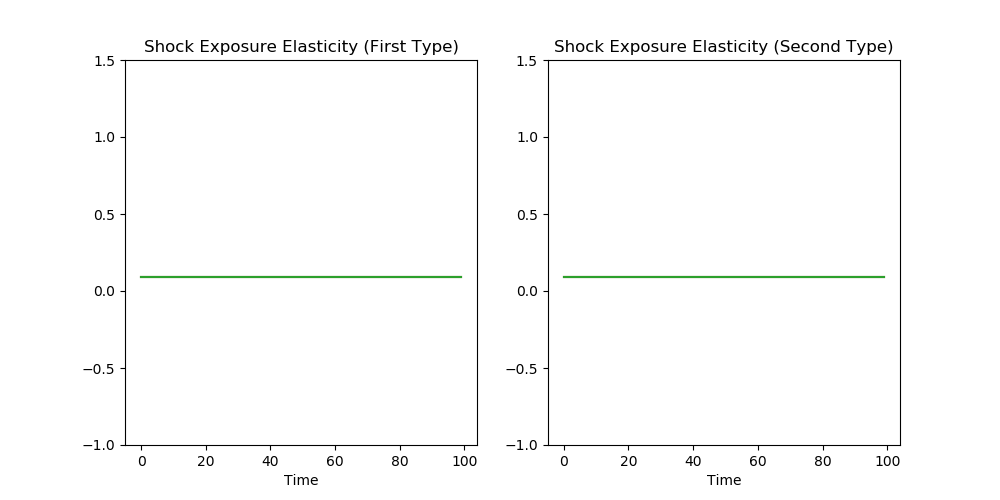
\includegraphics[scale=.4]{HK_expoC1.png}  \\
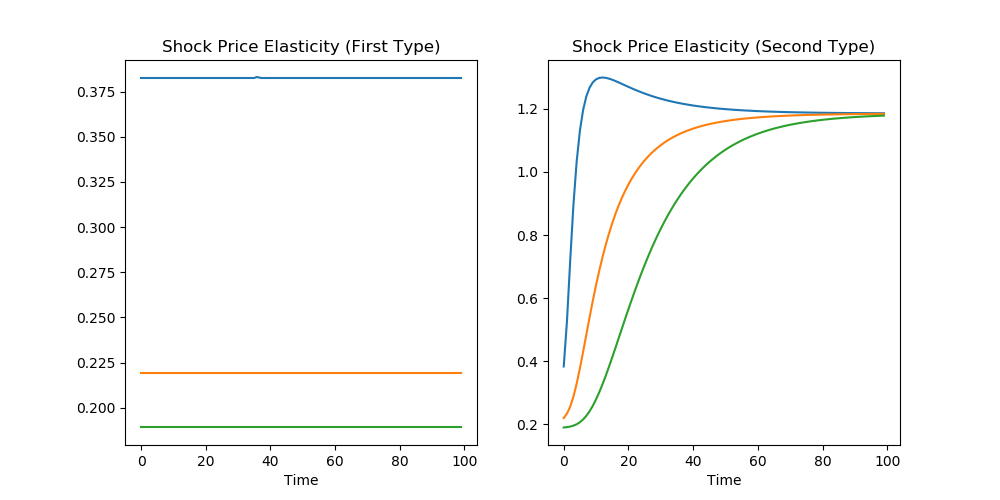
\includegraphics[scale=.4]{HK_priceC1.png} \\
\end{center}

The elasticities of the second cash flow $C^2$:
\begin{center}
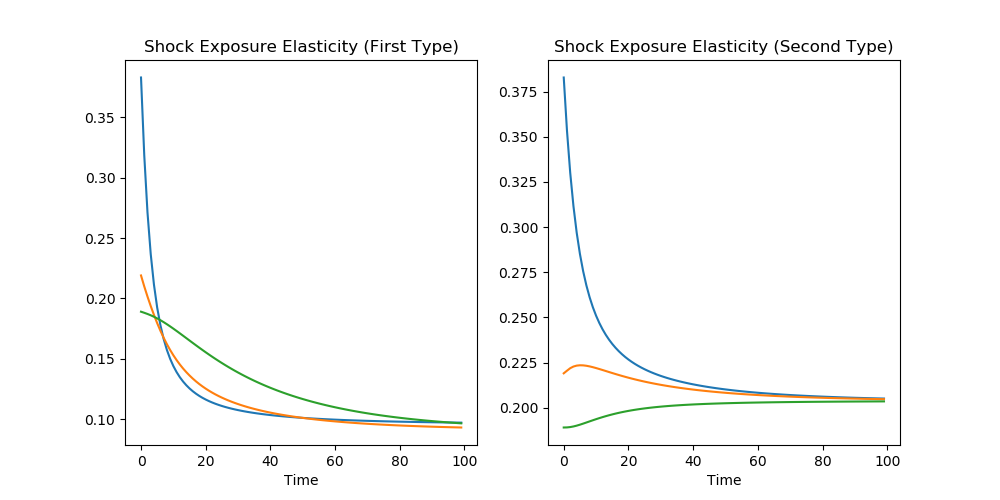
\includegraphics[scale=.4]{HK_expoC2.png}  \\
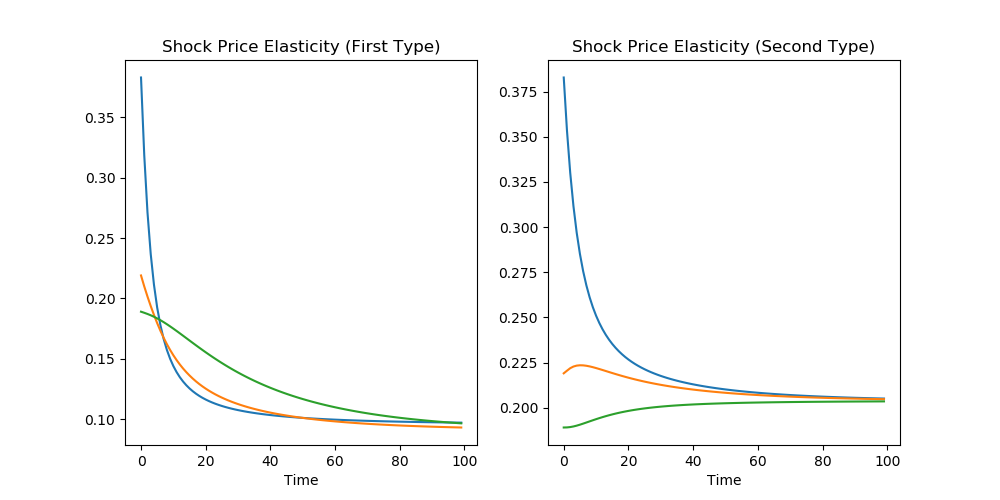
\includegraphics[scale=.4]{HK_priceC2.png} \\
\end{center}

\subsection{Bansal and Yaron (2004)}

This example \texttt{BansalYaron.py} is adapted from \citet{bansal_yaron}. Different from the example in \ref{HKExample}, the model has two state variables ($n = 2$) and three shocks ($k = 3$). The example computes elasticities for two utility functions (i.e. two SDFs).\\

The model has two state variables that follow stochastic processes:

\begin{align*}
dX^{[1]}_t &= -0.021 X^{[1]}_t dt + \sqrt{X^{[2]}_t} \begin{bmatrix} 0.00031 & -0.00015 & 0 \end{bmatrix} dW_t \\
dX^{[2]}_t &= -0.013 (X^{[2]}_t - 1) dt + \sqrt{X^{[2]}_t} \begin{bmatrix} 0 & 0 & -0.038 \end{bmatrix} dW_t \\
\end{align*}

Where aggregate consumption follows:
\begin{align*}
d\log{C_t} = 0.0015dt + X^{[1]}_t  dt + \sqrt{X^{[2]}_t} \begin{bmatrix} 0.0034 & 0.007 & 0 \end{bmatrix} dW_t
\end{align*}

Please note that the parameter settings and specific continuous-time specification comes from the handbook chapter of \cite{HHLR} to well approximate the dynamics used by \citet{bansal_yaron}. As in \citet{Hansen-2012}, we transform two of the shocks to the macroeconomy in order that one is permanent and the other is transitory. Furthermore, the intertemporal elasticity parameter is unity and the risk aversion parameter is $8$. \\

Suppose that the state dynamics are specified by

\begin{align*}
\mu(x) = \begin{bmatrix} \bar{\mu}_{11} & \bar{\mu}_{12} \\ 0 & \bar{\mu}_{22} \end{bmatrix} \begin{bmatrix}
x^{[1]} + \iota_1 \\  x^{[2]} + \iota_2 \end{bmatrix} \text{ and } \sigma(x) = \sqrt{x^{[2]}} \begin{bmatrix}
\bar{\sigma}_1 \\ \bar{\sigma}_2 \end{bmatrix}
\end{align*}

and the consumption dynamics take the following form:

\begin{align*}
\beta(x) = \bar{\beta}_{c,0} + \bar{\beta}_{c,1} (x^{[1]} - \iota_1) + \bar{\beta}_{c,2} (x^{[2]} - \iota_2) \text{ and } \alpha(x) = \sqrt{x^{[2]}} \bar{\alpha}_{c}
\end{align*}

We can recast the model by setting:

\begin{gather*}
\begin{bmatrix} \bar{\mu}_{11} & \bar{\mu}_{12} \\ 0 & \bar{\mu}_{22} \end{bmatrix} =
\begin{bmatrix} -0.021  & 0 \\ 0 & -0.013  \end{bmatrix},
\begin{bmatrix}
 \iota_1 \\  \iota_2 \end{bmatrix}  = \begin{bmatrix}
0 \\  -1 \end{bmatrix} \text{ and } \begin{bmatrix} \bar{\sigma}_1 \\  \bar{\sigma}_2 \end{bmatrix}  = \begin{bmatrix} 0.00031 & -0.00015 & 0 \\ 0 & 0 & -0.038 \end{bmatrix} \\
\bar{\beta}_{c,0} = 0.0015; \ \bar{\beta}_{c,1} = 1; \ \bar{\beta}_{c,2} = 0 \\
\bar{\alpha}_{c} = \begin{bmatrix} 0.0034 & 0.007 & 0 \end{bmatrix}
\end{gather*}

We compute the shock elasticities for both the recursive utility and power utility SDFs. The SDF of the recursive utility is given by:

\begin{align*}
S_t = \exp{(-\delta t)} \bigg( \frac{C_t}{C_0} \bigg)^{-1} \tilde{M}_t
\end{align*}

where $d\log{\widetilde{M_t}} =  - \frac{|\tilde{\alpha}|^2}{2} X^{[2]}_tdt + \sqrt{X^{[2]}_t} \tilde{\alpha} \cdot dW_t$. \\

When we take logs:
\begin{align*}
 d\log(S_t) &= -\delta dt - d\log(C_t) + \sqrt{X^{[2]}_t}\tilde{\alpha}\cdot dW_t - \frac{|\tilde{\alpha}|^2}{2}X^{[2]}_tdt \\
d\log(S_t) &= -\delta dt - \bigg[ \bar{\beta}_{c,0}dt + \bar{\beta}_{c,1} X^{[1]}_t dt + \bar{\beta}_{c,2} (X^{[2]}_t - 1)dt + \sqrt{X^{[2]}_t} \bar{\alpha}_c \cdot dW_t  \bigg] \\
&\ \ \ \ + \sqrt{X^{[2]}_t}\tilde{\alpha}\cdot dW_t - \frac{|\tilde{\alpha}|^2}{2}X^{[2]}_tdt \\
&= \bigg[ -\delta - \bar{\beta}_{c,0} - \bar{\beta}_{c,1} X^{[1]}_t - \bar{\beta}_{c,2} (X^{[2]}_t - 1) -  \frac{|\tilde{\alpha}|^2}{2}X^{[2]}_t \bigg] dt + \sqrt{X^{[2]}_t} (\tilde{\alpha} - \bar{\alpha}_c) dW_t
\end{align*}

Where $\tilde{\alpha} = (1 - \gamma) [(\bar{\sigma}_1)'\bar{v}_1 + (\bar{\sigma}_2)'\bar{v}_2 + \bar{\alpha}_c ]$ and $\bar{v}_1$ and $\bar{v}_2$ are computed by:

\begin{align*}
\bar{v}_1 &= \frac{-\bar{\beta}_{(c,1)}}{\bar{\mu}_{11} - \delta} \\
\bar{v}_2 &= \frac{{ - B \pm \sqrt {B^2 - 4AD} }}{{2A}}
\end{align*}

Where

\begin{align*}
A &= \frac{1 - \gamma}{2} (\bar{\sigma}^2_1 +  \bar{\sigma}^2_2) \\
B &= -\delta + \bar{\mu}_{22} + (1 - \gamma) ( \bar{\alpha}_c )' (\bar{\sigma}_2)' + 2 v_1 \frac{1 - \gamma}{2} \bar{\sigma}_1 \bar{\sigma}_2 \\
D &= \bar{\mu}_{12} \bar{v}_1 + \bar{\beta	}_{c,2} + (1 - \gamma)  ( \bar{\alpha}_c )' (\bar{\sigma}_1)'\bar{v}_1 + \frac{1 - \gamma}{2} ( \bar{\sigma}^{2}_1 \bar{v}^{2}_1 - \bar{\alpha}_c^2)
\end{align*}

We also compute the shock elasticities for power utility, whose SDF is given by

\begin{align*}
S_t = \exp{(-\delta t)} \bigg( \frac{C_t}{C_0} \bigg)^{-\gamma}
\end{align*} \\

Taking logs yields:

\begin{align*}
d\log(S_t) &= -\delta dt - \gamma d\log(C_t)  \\
&= -\delta dt - \gamma \bigg[ \mu_C(x)dt + \sqrt{X^{[2]}_t} \bar{\alpha}_c \cdot dW_t  \bigg] \\
&= \bigg[ -\delta - \gamma \mu_C(x) \bigg] dt + \gamma \sqrt{X^{[2]}_t} (- \bar{\alpha}_c) dW_t
\end{align*}

With these equations, we are ready to compute shock elasticities using the toolbox. We will compute the shock elasticities for starting points at the mean of $X^{[1]}$ and the 10th, 50th, and 90th percentiles of $X^{[2]}$ (3 starting points in total). In particular, some of the arguments for function \texttt{computeElas} are as follows - \\

Let $\tilde{S}$ be the total number of grid points:

\begin{itemize}
\item \texttt{model}
	\begin{itemize}
	\item[-] \texttt{muC}: a function that returns an $\tilde{S} \times 1$ numpy matrix
	\item[-] \texttt{sigmaC}: a function that returns an $\tilde{S} \times 3$ numpy matrix (remember, there are \textbf{3} shocks)
	\item[-] \texttt{muS}: a function that returns an $\tilde{S} \times 1$ numpy matrix
	\item[-] \texttt{sigmaS}: a function that returns an $\tilde{S} \times 3$ numpy matrix
	\item[-] \texttt{muX}: a function that returns an $\tilde{S} \times 2$ numpy matrix (there are \textbf{2} state variables)
	\item[-] \texttt{sigmaX} a list that contains $2$ functions, each of which returns an $\tilde{S} \times 3$ numpy matrix
	\end{itemize}

\item \texttt{x0}: a $3 \times 2$ matrix (there are \textbf{3} starting points and \textbf{2} dimensions)
\end{itemize}

You should expect the elasticities to look like:

\begin{center}
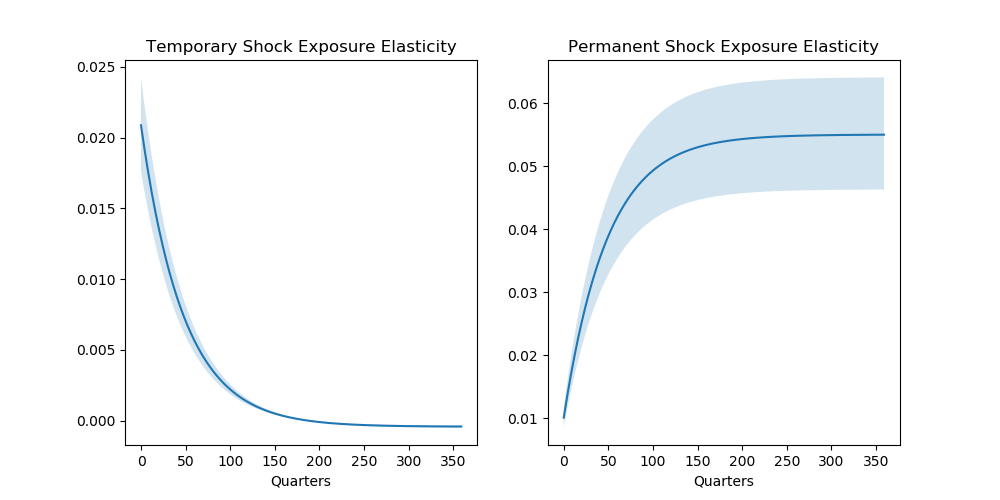
\includegraphics[scale=.4]{BY_shockExpo.png}  \\
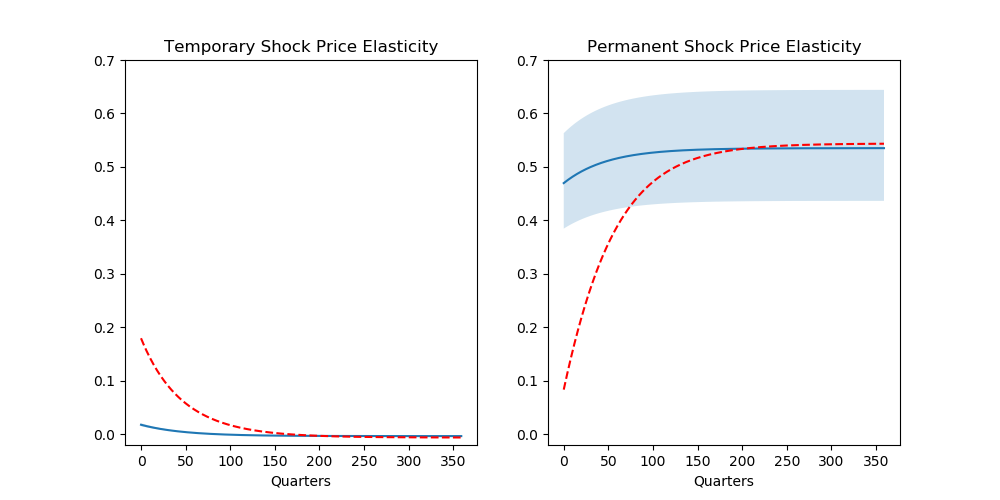
\includegraphics[scale=.4]{BY_shockPrice.png} \\
\end{center}

\subsection{One-Dimensional Hansen, Khorrami, and Tourre (2018)}

The file \texttt{test1DModel.py} demonstrates how to use the \texttt{modelSoln} class to solve the
one-dimensional version of the model in \citet{HKT}. In other words, the only
shock in this model is the TFP shock. Here we are only interested in using the
default parameters, so we create a model object and borrow default parameters from
the class.

\begin{minted}[
frame=lines,
framesep=2mm,
baselinestretch=1.2,
bgcolor=backcolour,
fontsize=\footnotesize,
linenos
]{python}
import mfr.modelSoln as m
params = m.paramsDefault.copy()
testModel = m.Model(params)
\end{minted}

Now that the model object has been defined, we call the \texttt{solve} command
to get a solution. In addition to solving the model, the program in
\texttt{test1DModel.py} does the following:

\begin{itemize}
    \item Computes the stationary density of the state variables with
    \texttt{computeStatDent()}
    \item Computes the mean and standard deviation of wealth and interest rates,
    using \texttt{computeMoments()}
    \item Computes the correlation of wealth share and interest rates using
    \texttt{computeCorrs()}
    \item Computes the shock elasticities starting at the 30th and 70th percentiles
    of wealth share using \texttt{computeShockElas()}. Using the same method, it
    also computes the shock elasticities starting at wealth share equal to 0.5.
\end{itemize}

Upon running the example file, you will see the following printed:
\begin{itemize}
    \item The solution info (\texttt{printInfo()})
    \item The parameters (\texttt{printParams()})
    \item The mean and standard deviation of wealth share and interest rate (the
    \texttt{moments} attribute after \texttt{computeMoments([`\wealthProg', `r'])})
    \item The correlation between the wealth share and interest rates (the
    \texttt{corrs} attribute after \texttt{computeCorrs([`\wealthProg', `r'])}).
\end{itemize}

\subsection{Two-Dimensional Hansen, Khorrami, and Tourre (2018)}

In \texttt{test2DModel.py} we examine the \citet{HKT} model with both the standard
TFP shock as well as a shock to aggregate TFP volatility. To effect this change,
we need to alter some of the default parameters.

\begin{minted}[
frame=lines,
framesep=2mm,
baselinestretch=1.2,
bgcolor=backcolour,
fontsize=\footnotesize,
linenos
]{python}
import mfr.modelSoln as m

params = m.paramsDefault.copy()

params['nV']           = 50
params['nWealth']      = 100
params['sigma_V_norm'] = 0.132
params['cov21']        = -0.1

testModel = m.Model(params)
\end{minted}

Note that since we are adding a second dimension with 50 grid points, we reduce
the number of grid points allocated to wealth share from the default 300 to 100
for computational simplicity. Recall that we only need to input the
\texttt{covij} parameter for $1 < i \leq k$ and $ 1 \leq j < i$ where $k$ is the
number of shocks, equal to 2 in this case.

From here, the example code is identical to that of \texttt{test1DModel.py}, except
that the elasticity starting points are different since they must be specified
for both of the state variables wealth share and aggregate volatility. We use
the 30th and 70th percentiles of wealth share and aggregate volatility first, then
use wealth share equal to 0.2 and 1.0 with aggregate volaility equal to 0.5 and
1.5. Refer to the documentation on \texttt{test1DModel.py} for more information.

\newpage

\section{Appendix}
\subsection{Parameters for \texttt{\modelSolnProg}}\label{append:Parameters}

\begin{ThreePartTable}
	\begin{TableNotes}
	\item[1] Any negative number for \texttt{\TFPhProg} means $-\infty$.
	\item[2] If \texttt{1}, experts' equity retention would be set as \texttt{\equityConstraintProg} everywhere; if \texttt{2}, the minimum of experts' equity retention is bounded from below by \texttt{\equityConstraintProg}, but it is not necessarily the case that equity retention is \texttt{\equityConstraintProg} everywhere.
	\item[3] We give an extensive explanation on this set of parameters in \ref{covParam}.
	\end{TableNotes}
            \begin{longtable}{|c|c|c|c|}
            \caption{Model parameters and their default values (last column)}\label{table:modelParams}\\
                \hline
                \multicolumn{4}{|c|}{\textbf{Model Parameters}} \\
                        \endfirsthead

        \endfoot

        \insertTableNotes         
        \endlastfoot
                \hline
                \texttt{\newbornRateProg} & \newbornRateSymbol & Fraction of newborns designated experts & 0.1 \\  \hline
                \texttt{\deathrateProg} & \deathrateSymbol & Birth/death rate & 0.02 \\ \hline
                \texttt{\persistGrowthProg} & \persistGrowthSymbol & Mean-reversion exogenous TFP growth & 0.252 \\ \hline
                \texttt{\persistStochasticVolProg} & \persistStochasticVolSymbol & Mean-reversion aggregate TFP volatility & 0.156 \\ \hline
                \texttt{\persistIdioVolProg} & \persistIdioVolSymbol & Mean-reversion idiosyncratic TFP volatility & 1.38 \\ \hline
                \texttt{\meanIdioVolProg} & \meanIdioVolSymbol & Mean idiosyncratic TFP volatility & 0.0 \\ \hline
                \texttt{\meanGrowthProg} & \meanGrowthSymbol & Mean exogenous TFP growth & 0.0 \\ \hline
                \texttt{\meanStochasticVolProg} & \meanStochasticVolSymbol & Mean ``normalized'' aggregate TFP volatility & 1.0\\ \hline
                \texttt{\discountRateEProg} & \discountRateESymbol & Expert rate of time preference & 0.05 \\ \hline
                \texttt{\discountRateHProg} & \discountRateHSymbol & Household rate of time preference & 0.05 \\ \hline
                \texttt{\TFPeProg} & \TFPeSymbol & Expert TFP & 0.14 \\ \hline
                \texttt{\TFPhProg} & \TFPhSymbol & Household TFP\tnote{1} & -1 \\ \hline
                \texttt{\inverseEISeProg} & \inverseEISeSymbol & Expert inverse EIS & 1.0 \\ \hline
                \texttt{\inverseEIShProg} & \inverseEIShSymbol & Household inverse EIS & 1.0 \\ \hline
                \texttt{\adjCostProg} & \adjCostSymbol & Adjustment cost parameter & 3.0 \\ \hline
                \texttt{\riskAverEProg} & \riskAverESymbol & Expert RRA & 1.0 \\ \hline
                \texttt{\riskAverHProg} & \riskAverHSymbol & Household RRA & 1.0 \\ \hline
                \texttt{\meanTFPVolProg} & \meanTFPVolSymbol & Mean TFP volatility & 0.04 \\ \hline
                \texttt{\growthVolProg} & \growthVolSymbol & Exogenous TFP growth volatility & 0.00 \\ \hline
                \texttt{\stochasticVolVolProg} & \stochasticVolVolSymbol & Volatility of ``normalized'' aggregate TFP volaility & 0.0 \\ \hline
                \texttt{\idioVolVolProg} & \idioVolVolSymbol & Volatility of ``normalized'' idiosyncratic TFP volaility & 0.0 \\ \hline
                \texttt{\equityConstraintProg} & \equityConstraintSymbol &  Minimum expert skin-in-the-game & 0.5 \\  \hline
                \texttt{\depreProg} & \depreSymbol & Depreciation rate & 0.05 \\ \hline
                \texttt{equityIss} & &\begin{tabular}{@{}c@{}}1: Expert’s constant equity retention constraint \\2: Minimum expert’s equity retention constraint\tnote{2} \end{tabular} & 2 \\ \hline
                \texttt{covij} &  & Coordinates of the correlation matrix of the shocks\tnote{3} &  0 \\ \hline
                \end{longtable}
\end{ThreePartTable}
\begin{table}
\centering
            \caption{Grid parameters and their default values (last column)}\label{table:gridParams}
            \begin{tabular}{|c|c|c|}
				\hline
                \multicolumn{3}{|c|}{\textbf{Grid Parameters}} \\
                \hline
                \texttt{numSds} & Number of standard deviations (for exogenous states) & 5 \\ \hline
                \texttt{\nWealthProg} & Number of grid points for wealth & 300\\ \hline
                \texttt{\nGrowthProg} & Number of points for growth  & 0\\ \hline
                \texttt{\nStochasaticVolProg} & Number of points for stochastic volatility & 0  \\ \hline
                \texttt{\nIdioVolProg} & Number of points for idiosyncratic volatility & 0 \\ \hline
                \texttt{\wealthMinProg} & Minimum for wealth grid & 0.01 \\ \hline
                \texttt{\wealthMaxProg} & Maximum for wealth grid & 0.99 \\ 
				\hline
                \end{tabular}
\end{table}

\begin{table}
\centering
            \caption{Numerical algorithm parameters and their default values (last column)}\label{table:algoParams}
            \begin{tabular}{|c|c|c|}
            \hline
                \multicolumn{3}{|c|}{\textbf{Numerical Algorithm Parameters}} \\
                \hline
                \texttt{method} & \begin{tabular}{@{}c@{}}1: Use the explicit scheme \\ 2: Use the implicit scheme\end{tabular} & 2 \\ \hline
                \texttt{dt} & Outer loop time step & 0.1 \\ \hline
                \texttt{dtInner} & Inner loop time step & 0.1 \\ \hline
                \texttt{tol} & Algorithm error tolerance & 0.00001 \\ \hline
                \texttt{innerTol} & Algorithm inner loop error tolerance & 0.00001 \\ \hline
                \texttt{verbatim} & \begin{tabular}{@{}c@{}} 1: Print out iteration information of the inner loop \\ -1: Do not print out iteration information of inner loop\end{tabular}& -1 \\ \hline
                \texttt{maxIters} & Maximum iterations allowed for the algorithm & 4,000 \\ \hline
                \texttt{maxItersInner} & Maximum iterations allowed for the algorithm inner loop & 2,000,000 \\  \hline
                \texttt{CGscale} & CG tolerance scaler & 1.0 \\
				\hline
                \end{tabular}
\end{table}

\begin{table}
\centering
            \caption{I/O parameters and their default values (last column)}\label{table:ioParams}
            \begin{tabular}{|c|c|c|}
            \hline
                \multicolumn{3}{|c|}{\textbf{I/O Parameters}} \\
                \hline
                \texttt{folderName} & Name of output folder to save all output & `model0' \\ \hline
                \texttt{overwrite} & `Yes' to overwrite output folder, `No' otherwise & `Yes' \\ \hline
                \texttt{exportFreq} & Data export frequency & 10000\\ \hline                
                \texttt{preLoad} & Folder from which the program loads guesses (optional) & empty\\ \hline
                \texttt{suffix} & Suffix of the \texttt{.dat} files (optional) & \texttt{`final'}\\ \hline
                \texttt{zetaEGuess} & guess for $\zeta_e$ (optional) & \texttt{np.array}  \\ \hline
                \texttt{zetaHGuess} & guess for $\zeta_h$ (optional) &  \texttt{np.array} \\ \hline
                \texttt{chiGuess} & guess for $\chi$ (optional) &  \texttt{np.array} \\ \hline
                \texttt{kappaGuess} & guess for $\kappa$ (optional) &  \texttt{np.array}  \\ \hline
                \end{tabular}
\end{table}
\subsection{Equilibrium Quantities and Variables in \cite{HKT}}\label{append:eqmQuant}
\begin{table}[H]
\centering
            \caption{Attributes related to the modeling freamwork in \cite{HKT}}\label{table:attributesHKT}
            \begin{tabular}{|l|l|}
				\hline
                \texttt{stateMat} & \begin{tabular}{@{}l@{}} a \texttt{pandas} dataframe that contains the grid \\ on which the model was solved. \end{tabular} \\ \hline
                \texttt{dent} & Stationary density of the model \\ \hline
                \texttt{FKmat} & \begin{tabular}{@{}l@{}} Feynman-Kac matrix, the transpose of which is \\ used for the stationary density \end{tabular} \\ \hline
                \texttt{marginals} & \begin{tabular}{@{}l@{}} Dictionary of marginal densities of \\ the state variables \end{tabular}\\ \hline
                \begin{tabular}{@{}l@{}} \texttt{apMoments}, \\ \texttt{macroMoments} \end{tabular} & \begin{tabular}{@{}l@{}}  Ergodic moments (mean and standard deviation)\\ of equilibrium quantities\end{tabular} \\ \hline
                \texttt{corrs} & Ergodic correlations of equilibrium quantities  \\ \hline
                \texttt{inverseCDFs} & Dictionary of inverse marginal CDFs of the state variables \\ \hline
                \texttt{params} & Parameters of the model  \\ \hline
                \texttt{gridSizeList} &List of grid sizes of the state variables  \\ \hline
                \end{tabular}
\end{table}
\begin{table}[H]
\centering
            \caption{Attributes useful in diagnosing the performance of the numerical algorithm}\label{table:methodsAlgoHKT}
            \begin{tabular}{|l|l|}
				\hline
                \texttt{timeOuterloop} &\begin{tabular}{@{}l@{}}  Time taken to solve \\ each iteration of the algorithm (outer loop) \end{tabular}  \\ \hline
                \texttt{timeLynSys} & \begin{tabular}{@{}l@{}} Time taken to solve \\the linear systems within each outer loop \end{tabular} \\ \hline
                \begin{tabular}{@{}l@{}} \texttt{errorsE}, \\ \texttt{errorsH} \end{tabular} & Error (i.e. time derivative) of experts and households per iteration  \\ \hline
                \begin{tabular}{@{}l@{}} \texttt{CGEIters}, \\ \texttt{CGHIters} \end{tabular} & \begin{tabular}{@{}l@{}} Number of steps taken for conjugate gradient \\ in each outer loop for experts' and households' value functions \end{tabular} \\ \hline
                \end{tabular}
\end{table}
\begin{table}[H]
\centering
            \caption{Methods to access the equilibrium quantities in \cite{HKT}}\label{table:methodsEqmQuantHKT}
            \begin{tabular}{|l|l|l|}
            \hline
                \texttt{W()} & Wealth share of the experts & $W$ \\ \hline
                \texttt{Z()} & Aggregate growth rate & $Z$ \\ \hline                
                \texttt{V()} & Stochastic volatility & $V$ \\ \hline
                \texttt{Vtilde()} & Idiosyncratic volatility & $\widetilde{V}$ \\ \hline
                \texttt{muW()}, \texttt{sigmaW()} & Drift and volatility of wealth share & $\mu_W$, $\sigma_W$ \\ \hline
                \texttt{muZ()}, \texttt{sigmaZ()}  & Drift and volatility of aggregate growth &  $\mu_Z$, $\sigma_Z$ \\ \hline
                \texttt{muV()}, \texttt{sigmaV()} & Drift and volatility of stochastic volatility & $\mu_V$, $\sigma_V$ \\ \hline
                \texttt{muVTilde()}, \texttt{sigmaVTilde()} & Drift and volatility of idiosyncratic volatility &  $\mu_{\widetilde{V}}$, $\sigma_{\widetilde{V}}$ \\ \hline
                \begin{tabular}{@{}l@{}} \texttt{piE\{\# shock\}()} \\ \texttt{piH\{\# shock\}()} \end{tabular} & \begin{tabular}{@{}l@{}}Risk prices of experts/households for shock $j$, \\indicated by \{\# shock\} \end{tabular}  &  $\pi_e^{j}, \pi_h^{j}$ \\ \hline
			  \begin{tabular}{@{}l@{}} \texttt{deltaE()} \\ \texttt{deltaH()}  \end{tabular} & Experts'/Households' Bonus Risk Premium &  $\Delta_e$, $\Delta_h$ \\ \hline
			  \begin{tabular}{@{}l@{}} \texttt{excessReturnKExperts()} \\ \texttt{excessReturnKHouseholds()}  \end{tabular} & Experts'/Households' Excess return on capital &   \begin{tabular}{@{}l@{}} $\mu_{R_e} - r$ \\  $\mu_{R_h} - r$\end{tabular} \\ \hline
			  \begin{tabular}{@{}l@{}} \texttt{chatE()} \\ \texttt{chatH()}  \end{tabular} & Experts'/Households' consumption to wealth ratio &  $\hat{c}_e$, $\hat{c}_h$ \\ \hline
			  \begin{tabular}{@{}l@{}} \texttt{xiE()} \\ \texttt{xiH()}  \end{tabular} & Experts'/Households' value functions &  $\xi_e$, $\xi_h$ \\ \hline
                \texttt{muQ()}, \texttt{sigmaQ()} & Drift  and volatility of capital price &  $\mu_q$, $\sigma_q$ \\ \hline
                \texttt{kappa()} & Experts' capital retention &  $\kappa$ \\ \hline
                \texttt{chi()} & Experts' equity holdings &  $\chi$ \\ \hline
                \texttt{r()} & Interest rate &  $r$ \\ \hline
                \texttt{q()} & Capital price &  $q$ \\ \hline
                \texttt{I()} & Investment rate &  $I$ \\ \hline
                \texttt{CoverI()} & Consumption-to-investment ratio &  $C/I$ \\ \hline
                \texttt{IoverK()} & Investment-to-capital ratio &  $I/K$ \\ \hline
                \texttt{CoverK()} & Consumption-to-capital ratio &  $C/K$ \\ \hline
                \texttt{IoverY()} & Investment-to-output ratio &  $I/Y$ \\ \hline
                \texttt{CoverY()} & Consumption-to-output ratio &  $C/Y$ \\ \hline
                \texttt{Ieverage()} & Experts' leverage &  $\kappa \chi / W$ \\ \hline
                \texttt{muK()}, \texttt{sigmaK()}  & Drift and volatility of capital &  $\mu_k$, $\sigma_k$ \\ \hline
                \texttt{muY()}, \texttt{sigmaY()}  & Drift and volatility of aggregate growth &  $\mu_Y$, $\sigma_Y$ \\ \hline
                \texttt{piETilde()}, \texttt{piHTilde()}  & Experts' and households' idiosyncratic risk prices &  $\tilde{\pi}_e$, $\tilde{\pi}_h$ \\ \hline
                \begin{tabular}{@{}l@{}} \texttt{muC()} \\ \texttt{muCe()}, \texttt{muCh()}  \end{tabular} & \begin{tabular}{@{}l@{}} Drift of aggregate consumption, \\ experts' consumption, and households' consumption  \end{tabular}  &   \begin{tabular}{@{}l@{}} $\mu_C$ \\ $\mu_{C_e}$ \\ $\mu_{C_h}$ \end{tabular}  \\ \hline
                \begin{tabular}{@{}l@{}} \texttt{sigmaC()} \\ \texttt{sigmaCe()}, \texttt{sigmaCh()}  \end{tabular} & \begin{tabular}{@{}l@{}} Volatility of aggregate consumption, \\ experts' consumption, and households' consumption  \end{tabular}  &   \begin{tabular}{@{}l@{}} $\sigma_C$ \\ $\sigma_{C_e}$ \\ $\sigma_{C_h}$ \end{tabular}  \\ \hline
                \texttt{muSe()}, \texttt{sigmaSe()}  & Drift and volatility of experts' SDF &  $\mu_{S_e}$, $\sigma_{S_e}$ \\ \hline
                \texttt{muSh()}, \texttt{sigmaSh()}  & Drift and volatility of households' SDF &  $\mu_{S_h}$, $\sigma_{S_h}$ \\ \hline
                \end{tabular}
\end{table}

\section{Change Log}
\subsection{Version 0.1.1}
\begin{itemize}
\item Added the option to compute shock elasticities in the Jupyter GUI by perturbing wealth share (\wealthSymbol)
\item Added plots of return on capital diffusion ($\sigma_R$) in the Jupyter GUI
\item Added plots of risk price differences ($\pi_e - \pi_h$) in the Jupyter GUI
\item Changed \texttt{init\_notebook\_mode(True)} to \texttt{init\_notebook\_mode(False)} so that the GUI can display charts when offline
\item Removed \texttt{displayModeBar = True} in functions that involve Plotly so that Plotly plots won't display the modebar by default
\item Fixed bug where when preloading $\kappa$ and $\chi$ as solutions
\item In \texttt{.computeStatDent()} of \texttt{mfr.modelSoln}, added the feature to export stationary density and preload stationary density. Added the argument \texttt{forceCompute} so that the user can opt to compute stationary density even if the density is already computed
\end{itemize}
\subsection{Version 0.1.2}
\begin{itemize}
\item Fixed the calculation of experts' capital retention ($\kappa$) and experts' equity holding ($\chi$) when 1) households' productivity ($a_h$) equals experts' productivity ($a_e$), and 2) there is no idiosyncratic risk state.
\item Added a new method \texttt{.calDriftDiffusion()} to \texttt{mfr.modelSoln}. Advanced users can pass into any $f(X)$ (a function of state $X$, defined on the state grids. For example, f(X) could be model.muCe()). The method will return the drift and diffusion coefficients of $f(X)$, which are also defined on the state grids. 
\item Fixed y-axis scaling issue where when showing exposure elasticity plots in the Jupyter GUI.
\end{itemize}

\newpage
\bibliographystyle{jf}
\bibliography{ref}

\end{document}
